% !TeX program = pdflatex
% !TeX encoding = UTF-8
% !TeX spellcheck = pt_BR
\documentclass[12pt,a4paper,final]{article}
\usepackage[utf8]{inputenc}
\usepackage[brazil]{babel}
\usepackage{lmodern}
\usepackage{csquotes}

% Links nas referência cruzada no documento.
% Ajuda a navegação (principalmente no índice).
\usepackage[unicode]{hyperref}
\hypersetup{
    %hidelinks,   % Comente aqui para exibir os links
    colorlinks, % Descomente esse se comentar o de cima
    linkcolor={red!50!black},
    citecolor={blue!50!black},
    urlcolor={blue!80!black}
}

\usepackage[pdftex,dvipsnames,table,xcdraw]{xcolor}

% Melhorias na justificação do texto e
% pequenos ajustes em fontes e alinhamentos. 
\usepackage[T1]{fontenc}
\usepackage{microtype}

% Faz com que linhas orfãs sejam fortemente
% penalizadas. Mas é impossível evitá-las
% completamente.
\clubpenalty=9996
\widowpenalty=9999

% Permite o alinhamento horizontal de várias
% equações, assim elas não tomam muito espaço
% quando são muito pequenas.
\usepackage{tabularx}

% Símbolos diferentes para o texto, como setas →,
% símbolos de copyright e trademark, euro, etc.
% Não é muito útil, mas de vez em quando ajuda.
% Ao invés do comando do latex, dá pra usar o
% caractere em UTF-8 diretamente.
\usepackage{textcomp}

% Pequenos símbolos que são úteis (às vezes)
% como checkmark.
\usepackage{bbding}

% Ajustes finos em comandos do Latex
\usepackage{etoolbox}

% Permite criar formatações específicas, controla
% numerações e produz índices para teoremas e hipóteses.
\usepackage{amsthm}
\usepackage{thmtools}

\declaretheoremstyle[spaceabove=1.5ex,
                     spacebelow=0ex,
                     headindent=\parindent,
                     headformat=\MakeUppercase{\NAME} \NUMBER:\MakeUppercase{\NOTE},
                     notebraces={}{},
                     headpunct=:,
                     bodyfont=\itshape,
                     name=Hipótese]
                     {hypostyle}
\declaretheorem[style=hypostyle]{hypothesis}

% Para listagens de programação ou 
% textos onde a formatação importa
\usepackage{listings}
\lstset{
	inputencoding=utf8,
    extendedchars=true,
	framextopmargin=2pt,
    framexbottommargin=2pt,    
    literate={á}{{\'a}}1
             {ã}{{\~a}}1
             {é}{{\'e}}1
             {í}{{\'i}}1
             {ç}{{\c{c}}}1
             {Ç}{{\c{C}}}1,
}
\renewcommand{\lstlistingname}{Listagem}% Listing -> Listagem
\renewcommand{\lstlistlistingname}{Lista de \lstlistingname s}% List of Listings -> Lista de Listagens

% Permite colocar figuras lado a lado ou
% fazer posicionamentos arbitrários
\usepackage[lofdepth,lotdepth]{subfig}

% Permite o uso da opção "frame" em "includegraphics"
% para fazer uma borda na imagem
\usepackage[export]{adjustbox}

% Para inserir gráficos e imagens
\usepackage{graphicx}
% Diretório padrão para figuras
\graphicspath{ {images/} }

\usepackage{abnt-alf}
\usepackage[top=3cm,bottom=2cm,left=3cm,right=2cm]{geometry}
\usepackage{indentfirst}

% Adiciona o comando \source para citar fontes abaixo
% de figuras. Muito útil!
\usepackage{caption}
\newcommand{\source}[1]{\vspace{-10pt} \caption*{Fonte: {#1}} }

% Facilita o copy 'n paste no PDF
% Remove ligaturas na cópia
\input{glyphtounicode}
\pdfgentounicode=1

% Usado para comentar grandes porções do texto
% com \begin{comment} \end{comment}
\usepackage{comment}

% Para quebrar células de tabelas e melhorar
% a formatação.
% Meio complicado para fazer apenas isso,
% mas funciona.
\usepackage{array}
\usepackage{makecell}

\renewcommand\theadalign{cb}
\renewcommand\theadfont{\bfseries}
\renewcommand\theadgape{\Gape[4pt]}
\renewcommand\cellgape{\Gape[4pt]}

% Texto colorido e afins. Bom para TODO notes
\usepackage{xargs}
\usepackage[normalem]{ulem}
\useunder{\uline}{\ul}{}

% Todo notes.
% Muito útil para deixar anotações enquanto se está
% construindo o texto, depois dá para remover e onde
% quebrar são comentário que devem ser removidos.
% Para remover os comentários do PDF final, basta
% colocar 'disable' na lista de argumentos do pacote:
% \usepackage[disable]{todonotes}
\usepackage[obeyFinal,colorinlistoftodos,prependcaption,textsize=tiny]{todonotes}
\newcommandx{\question}[2][1=]{\todo[linecolor=red,backgroundcolor=red!25,bordercolor=red,#1]{#2}}

\newcommandx{\change}[2][1=]{\todo[linecolor=blue,backgroundcolor=blue!25,bordercolor=blue,#1]{#2}}

\newcommandx{\info}[2][1=]{\todo[linecolor=OliveGreen,backgroundcolor=OliveGreen!25,bordercolor=OliveGreen,#1]{#2}}

\newcommandx{\draft}[2][1=]{\todo[linecolor=Plum,backgroundcolor=Plum!25,bordercolor=Plum,#1]{#2}}

\newcommandx{\thiswillnotshow}[2][1=]{\todo[disable,#1]{#2}}
\reversemarginpar
% END Todo notes.

% Notações matemáticas usadas na dissertação.
% Usando elas é possível trocar toda a notação
% apenas mexendo nesse arquivo. Lembre sempre
% de olhá-lo antes de fazer equações.
% Para fórmulas matemáticas
\usepackage{amsmath}
\usepackage{amssymb}
\usepackage{mathtools}

% Para setas usadas em fórmulas dos grafos
\usepackage{MnSymbol}

% Notações matemáticas usadas com frequência no texto.
% Isso possui três vantagens:
% 1 - Dá menos trabalho digitar as fórmulas
% 2 - Dá mais consistência à notação no trabalho
% 3 - Se mudar de ideia qto à notação, é só trocar aqui
%     e o trabalho todo fica certo.
% Notação matemática
\newcommand{\R}{\mathbb{R}} % Reais
\renewcommand\vec{\mathbf} % vetor como negrito
\newcommand{\avg}[1]{\left\langle #1 \right\rangle} % ... média
\newcommand{\defn}{\coloneqq} % Usamos "=", ":=" ou "\equiv?"
\newcommand{\noloop}[1]{#1^\nlcirclearrowleft} % ... sem loops
% Redes direcionadas
\newcommand{\linkin}[1]{#1^\leftarrow} % ... entrada
\newcommand{\linkout}[1]{#1^\rightarrow} % ... saída
\newcommand{\linkboth}[1]{#1^\leftrightarrow} % ... direcionada
% Redes ponderadas e direcionadas
\newcommand{\win}{w^\leftarrow} % peso e direção de entrada
\newcommand{\wout}{w^\rightarrow} % peso e direção de saída
\newcommand{\weighted}[1]{#1^w} % ... com pesos
\newcommand{\weighteddir}[1]{#1^{w\rightarrow}} % ... com peso e direção
% Reciprocidade
\newcommand{\recin}[1]{#1^\leftlsquigarrow} % ... entrada não-recíproca
\newcommand{\recout}[1]{#1^\leadsto} % ... saída não-recíproca
\newcommand{\recboth}[1]{#1^\leftrightsquigarrow} % ... recíproca
% Capacidades
\newcommand{\capac}{\textit{cap}}

\begin{document}

% CAPA
\pagestyle{empty}
\begin{center}
\large  \textbf{UNIVERSIDADE PRESBITERIANA MACKENZIE}
\large  \textbf{PROGRAMA DE PÓS-GRADUAÇÃO EM}\\
\large  \textbf{ENGENHARIA ELÉTRICA E COMPUTAÇÃO}\\
\vskip 2.0cm
\textbf{\large Ronie Miguel Uliana}\\
\vskip 3.4cm
\setlength{\baselineskip}{1.5\baselineskip}
\textbf{\MakeUppercase{\large Compressão de Fluxo para Identificação de Fronteiras de Carreiras}}\\
\vskip 4.0cm
\end{center}
\hfill{\vbox{\hsize=8.5cm\noindent\strut
Documento de Qualificação apresentado ao \break
Programa de Pós-Graduação em Engenharia \break
Elétrica e Computação da Universidade \break
Presbiteriana Mackenzie como parte dos \break
requisitos para a obtenção do título de \break
mestre em Engenharia Elétrica e Computação.}\\
\strut}
\vskip 3.0cm
\textbf{\normalsize Orientador: Prof. Dr. Leandro Nunes de Castro}\\
\vskip 2.0cm
\begin{center}
São Paulo\\
2017\\
\end{center}

% RESUMO
\newpage
\thispagestyle{plain}
\pagenumbering{roman}
\begin{center}
\large
\textbf{RESUMO}
\end{center}
\renewcommand{\baselinestretch}{0.6666666}
A carreira profissional corresponde à jornada de um indivíduo pelo trabalho, sendo impactada diretamente pela cultura, formação e interesses pessoais. As movimentações de carreira representam passagens entre diferentes trabalhos (por exemplo, empresas ou cargos) e invariavelmente geram expectativas e angústias nos profissionais. A VAGAS.com é uma das principais empresas de recrutamento on-line do Brasil, possuindo o histórico de movimentação de carreira de mais de 10 milhões de brasileiros em mais de 8 mil cargos diferentes. A empresa criou um serviço gratuito, denominado Mapa de Carreiras (MCar), que exibe as principais trajetórias profissionais do mercado obtidas a partir de dados informados nos currículos cadastrados. Esse projeto de pesquisa utiliza uma área do conhecimento que vem se desenvolvendo muito ao longo das duas últimas décadas, denominada Ciência de Redes, para realizar um estudo analítico sobre o MCar. O MCar é uma rede complexa direcionada e ponderada, na qual os nós representam as ocupações profissionais e os arcos indicam a quantidade de profissionais que percorreram o caminho entre cada par de ocupações. Nesse contexto essa dissertação propõe contribuições em duas frentes: 1) proposição de adaptações e derivações de modelos de redes aleatórias existentes para que comportem as características do MCar; e 2) estudos analíticos que permitam compreender ou inferir movimentações profissionais a partir dos dados reais do Mapa de Carreiras.

%%\\[0.5cm]
\begin{flushleft}
{\bf Palavras-chave:} \it{redes, grafos, carreira, ocupações}
\end{flushleft}

% SUMÁRIO
\newpage
\thispagestyle{empty}
\tableofcontents

% DESENVOLVIMENTO
\newpage
\pagestyle{plain}
\pagenumbering{arabic}
\renewcommand{\baselinestretch}{1.5}
\normalsize

\listoftodos[Notas]

%====================================
\section{INTRODUÇÃO}
%====================================

Ao longo da vida profissional é comum para o indivíduo passar por diversas movimentações na carreira. Um estudante de engenharia pode iniciar como Trainee em uma empresa e progredir para Engenheiro, Supervisor de Obras e Diretor de Engenharia. Na área de computação é possível ver um Programador se tornar Analista-Programador, Coordenador de Desenvolvimento, Gerente de Projetos, chegando a Diretor. Esses são casos em que a movimentação de carreira segue um padrão mais tradicional de progressão baseado no plano de carreira de uma organização. Por outro lado, há situações extremas de transições de carreira na qual um Analista-Programador resolve se tornar um Chef de Cozinha ou um Eletricista Industrial passa a atuar como Web Designer. Em qualquer um dos casos, as movimentações de carreira são sempre uma etapa de grande relevância profissional e que, ao mesmo tempo, podem causar estresse, insegurança e alguns desconfortos pelos novos desafios que surgirão.

A movimentação profissional é discutida por modelos como os da \textit{Carreira Proteana} e \textit{Carreira sem Fronteiras}. Esses modelos advogam um distanciamento das carreiras ditadas pelo organograma das empresas em favor de trajetórias com foco maior no indivíduo~\cite{Bendassolli2009-bg}. A carreira proteana coloca o indivíduo, e não as organizações, como protagonista da trajetória profissional, onde seus valores são usados na decisão dos próximos passos e o sucesso é subjetivo e medido pela satisfação pessoal~\cite{Hall2004-ke}. A carreira sem fronteiras, por sua vez, acontece quando a trajetória se faz independente das organizações ou hierarquias. Essas carreiras são caracterizadas por passagens por múltiplas empresas ou mudanças na especialidade do indivíduo~\cite{Arthur1994-qq}.

No entanto, o movimento de uma pessoa entre ocupações profissionais não é simples. A capacitação do indivíduo, a atratividade da nova ocupação e o próprio conhecimento de que uma transição é possível a tornam mais fácil ou difícil para os profissionais. Quando essa transição é percebida como uma barreira por um número suficiente de pessoas, surge uma \textit{fronteira de carreira}~\cite{Gunz2007-hr}.

Este projeto de pesquisa utiliza o conceito de fronteira de carreira~\cite{Gunz2007-hr}, um banco de dados real com 23 milhões de experiências profissionais~\cite{VAGAS_Tecnologia2014-yv} e técnicas de detecção de comunidades em redes~\cite{Rosvall2009-sd,Edler2017-kt} para encontrar as fronteiras de carreira no mercado de trabalho brasileiro, discutir e entender sua estrutura.

Modelando o problema como um grafo e usando as técnicas de Ciência de Redes, o estudo revela onde estão as fronteiras de carreira e propõe o conceito de \textit{Ilha Ocupacional} para caracterizá-lo. O termo sugere que esses grupos não são formados por alguma característica intrínseca comum entre seus membros, mas sim pelo distanciamento dos outros membros, como proposto por \citeonline{Abbott1995-ft}. Isso significa que as ilhas são uma função da dificuldade da movimentação profissional inter-ilhas e da facilidade de movimentação intra-ilha, independente de atributos derivados de seu conteúdo ou significado.

O estudo prossegue analisando a composição a composições das ilhas e apresenta \textit{insights} sobre sua estrutura. O resultado obtido pode ser usado para o refinamento de teorias sobre carreira, como uma classificação natural para as ocupações baseada na movimentação profissional ou como subsídio para o planejamento de carreiras.

A principal contribuição desse trabalho está em tornar concreto o conceito de \textit{fronteiras de carreira}, revelando a estrutura da movimentação profissional no Brasil. Explorando esse conceito, o trabalho caracteriza a topologia das ilhas ocupacionais e propõe o conceito de \textit{Polos Ocupacionais} como ocupações que possuem papel crucial na estrutura. A topologia encontrada na maior parte das ilhas tende a um formato estrelado, sugerindo que a atuação nos polos afeta a ilha como um todo.

A presença de uma ilha gigante nos resultados fornece indícios que suportam o modelo de \textit{Carreira sem Fronteiras}, ao mesmo tempo em que indica que ela não abrange todos os segmentos profissionais.

Como essa pesquisa é baseada somente nos dados encontrados nos currículos, não é possível responder o que motiva os profissionais nos comportamentos observados, mas é possível afirmar que eles ocorrem. Um estudo dos porquês e das motivações necessita de um aprofundamento psicológico e sociológico que essa pesquisa é incapaz de atingir. Por outro lado, futuros trabalhos nesse sentido podem se apoiar nos resultados aqui obtidos para expandir a compreensão desses comportamentos.

(EXPANDIR) Outras pesquisas\ldots

% Ronie: Não é bem verdade. Acabei achando outro trabalhos que utilizam redes profissionais, principalmente do LinkedIn. Melhor expandir depois para mencioná-los.
Existem diversas pesquisas sobre movimentação profissional, principalmente sobre os fatores que motivam a mudança, como os expostos por~\citeonline{Ng2007-zp}. Porém, nenhum trabalho pôde ser encontrado analisando redes profissionais sob a ótica da Ciência de Redes, tornado-se outro ponto onde esse trabalho possui contribuições.

Como contribuição final, a movimentação de profissionais é um ponto de interesse para pessoas, empresas e governo. Pessoas desejam saber onde podem chegar, empresas se interessam pela contratação e evolução de seus colaboradores e o setor público traça planos para suprir mão de obra onde ela é insuficiente ou criar oportunidades de trabalho onde ela é abundante. A pesquisa presente traz uma maior compreensão sobre como essa movimentação ocorre e quais sua limitações.

Na seção X \ldots (EXPANDIR)

%====================================
\section{CIÊNCIA DE REDES}
%====================================

A Ciência de Redes (\textit{Network Science}) é uma área de estudo recente. Apesar do estudo matemático de grafos remontar ao século 18, com Leonhard Euler, o estudo de redes tem-se intensificado, culminando em um surto de interesse no começo do século 21 com os trabalhos de Watts-Strogatz e Barabási-Albert~\cite{Watts1998-wt,Barabasi1999-sn} sobre redes complexas.

Redes complexas são grafos com características topológicas que não ocorrem em redes simples ou aleatoriamente geradas, mas que aparecem quando sistemas reais são modelados como grafos, como a conectividade da Internet ou a rede de amigos nas redes sociais~\cite{Barabasi2016-rn}. Uma dessas características é, por exemplo, a presença de \textit{hubs}. Nós com um número anormalmente alto de conexões comparativamente com outros nós da rede.

Um marco para a consolidação da disciplina ocorreu em 2005 com o aval de órgãos governamentais quanto a sua utilidade como ciência. Nesse ano, o exército Norte-Americano solicitou ao \textit{United States National Research Council} um estudo sobre a aplicabilidade da emergente \enquote{Ciência de Redes}. O relatório~\cite{National_Research_Council2006-lv} destaca a relevância do campo em diversas áreas e levanta seus desafios. Nos anos seguintes foram fundados centros de estudos de Ciência de Redes nas universidades norte-americanas com investimentos dos laboratórios de pesquisa do exército~\cite{Maxwell2009-kq}.

O \citeonline{National_Research_Council2006-lv} define a Ciência de Redes como \enquote{o estudo da representação em rede de fenômenos físicos, biológicos e sociais levando a modelos preditivos desses fenômenos}~\footnote{Em tradução livre, \enquote{the study of network representations of physical, biological, and social phenomena leading to predictive models of these phenomena.}}.

Segundo \citeonline{Barabasi2016-rn}, como disciplina, a Ciência de Redes se diferencia de uma abordagem tradicional pelos seguintes pontos:

\begin{description} \label{desc:ciencia-de-redes}
	\item[\textit{Interdisciplinar}.] A Ciência de Redes é terreno comum para diversas disciplinas, como Biologia (com redes de proteínas), Sociologia (com redes sociais), Computação (com redes de comunicações e algoritmos), entre outras. Apesar de divergirem em essência e propósito, as redes que são seu objeto de estudo compartilham características e propriedades.
    
    \item[\textit{Empírica}.] A Ciência de Redes foca em dados reais e no propósito de uso das redes. Modelos teóricos são confrontados com dados reais para avaliação de sua utilidade na descoberta de propriedades relevantes das redes.
    
    \item[\textit{Matemática e Quantitativa}.] A Ciência de Redes baseia-se fortemente na Teoria de Grafos, na Estatística e em Algoritmos para criação de modelos e sua avaliação. A descoberta de princípios gerais de organização das redes só é possível com uma sólida base formal Matemática.
    
    \item[\textit{Computacional}.] Redes reais por vezes são de grande tamanho, com milhares ou milhões de nós, como a Internet ou as relações entre trabalho e pessoas. As características de algumas topologias, como a distribuição dos graus dos nós, somente são distinguíveis quando o número de nós e conexões é bastante grande. Adicionalmente, as análises comparativas com modelos nulos pressupõe a geração de grandes quantidades de redes aleatórias de composição similar às redes em estudo, um trabalho que não é possível sem o uso intensivo de computadores. Algoritmos e técnicas de processamentos de grandes volumes de dados são ferramentas essenciais para esses estudos.
\end{description}

%====================================
\subsection{Conceitos de Redes}

É preciso descrever os conceitos utilizados em redes para compreensão desse trabalho. Apesar de serem básicos em Teoria de Grafos, uma breve descrição é oferecida nas seções seguintes para completude dessa obra.

Um \textit{grafo} ou \textit{rede} é uma abstração usada quando o foco do estudo está no relacionamentos entre entidades. Nessa abstração, outras características das entidades que não o relacionamento são descartadas. Redes são representadas graficamente por formas geométricas, em geral pequenos círculos para representar as entidades, conectados por linhas representando os relacionamentos (Figura~\ref{fig:exemplo-tipos-grafo}).

\begin{figure}[ht]
    \centering
    \subfloat[][simples] {
        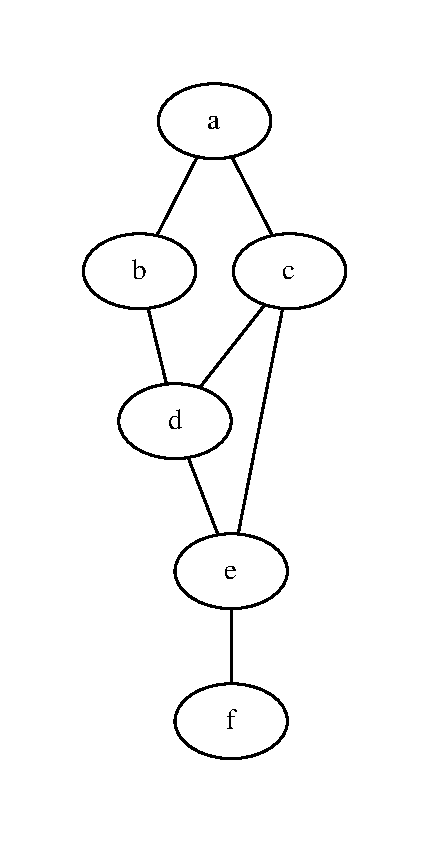
\includegraphics[scale=0.5]{simple.pdf}
        \label{fig:exemplo-grafo-simples}
    }
    \subfloat[][direcionado] {
        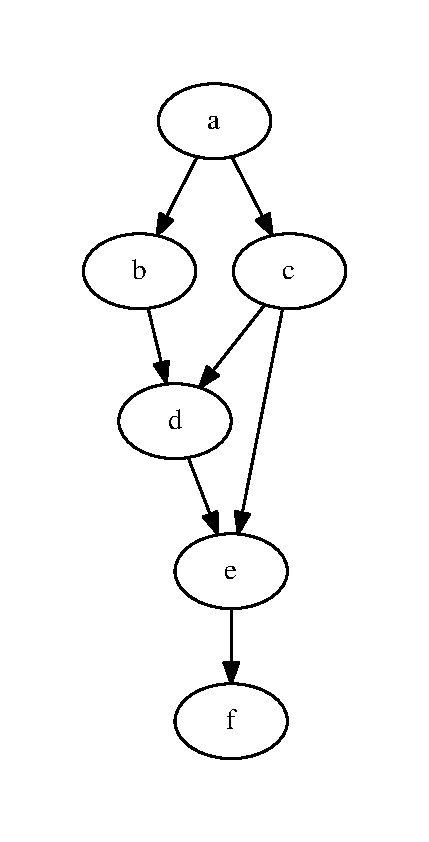
\includegraphics[scale=0.5]{directed.pdf}
        \label{fig:exemplo-grafo-direcionado}
    }    
    \subfloat[][ponderado] {
        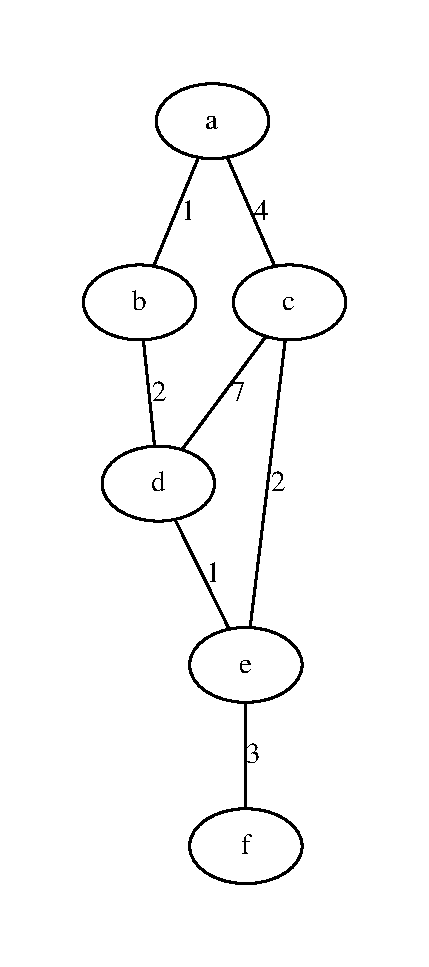
\includegraphics[scale=0.44]{weighted.pdf}
        \label{fig:exemplo-grafo-ponderado}
    }    
    \caption{Redes ou Grafos}
    \label{fig:exemplo-tipos-grafo}
    \source{Elaboração do autor}
\end{figure}

As entidades da rede são chamadas \textit{nós} ou \textit{vértices}, enquanto os relacionamentos são chamados \textit{conexões} ou \textit{arestas}. Os artigos científicos sobre Ciência de Redes dão preferência aos termos \textit{rede}, \textit{nó} e \textit{conexão}, enquanto no campo da Teoria de Grafos os termos são \textit{grafo}, \textit{vértice} e \textit{aresta}~\cite[p.~45]{Barabasi2016-rn}. Nesse trabalho deu-se preferência pelos termos usados em Ciência de Redes, no entanto, os termos de Teoria de Redes, quando usados, são considerados sinônimos.

Quando os relacionamentos possuem uma certa direção eles formam \textit{redes direcionadas} (Figura~\ref{fig:exemplo-grafo-direcionado}). Por exemplo, uma rede que representa as trocas de presentes natalinos é uma rede em que há \textit{direção}, o presente é dado de uma pessoa \textit{para} outra. Em outros casos, quando não há uma direção no relacionamento, a rede é chamada \textit{não-direcionada}. Por exemplo, em uma rede de relacionamentos os indivíduos se conhecem mutuamente. Uma conexão direcionada é por vezes chamada \textit{arco}.

Se a intensidade do relacionamento é relevante as conexões ganham um \textit{peso} (Figura~\ref{fig:exemplo-grafo-ponderado}). Seu significado depende da rede em questão. Por exemplo, em uma rede de transportes o peso pode significar a distância entre locais de entrega, em uma rede de dados pode significar o volume do tráfego entre os pontos, e em uma rede social pode significar o número de mensagens trocadas entre duas pessoas. Redes onde existe a presença de conexões com peso são chamadas \textit{redes ponderadas}.

Algumas redes permitem múltiplas conexões entre dois nós (Figura~\ref{fig:exemplo-grafo-multiplo}). Por exemplo, em uma rede de ligações telefônicas é possível representar cada ligação por uma conexão diferente, duas pessoas que troquem ligações seriam representadas por dois nós com diversas conexões entre si, uma para cada ligação feita. Redes que permitem múltiplas conexões são chamadas \textit{multigrafos}. Dependendo do fenômeno sendo modelado, multigrafos podem ser representados por redes ponderadas, em especial redes onde o relacionamento significa fluxo~\cite{Newman2004-by}.

\begin{figure}[ht]
    \centering
    \subfloat[][laços e direção] {
        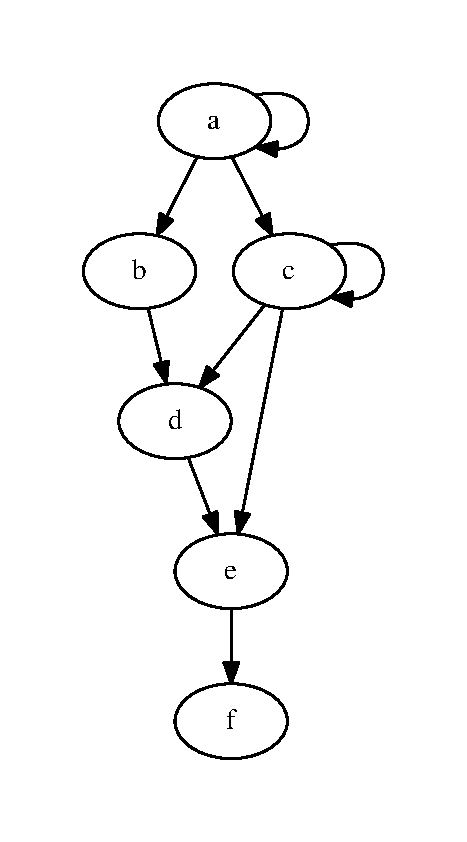
\includegraphics[scale=0.5]{loop.pdf}
        \label{fig:exemplo-grafo-laco}
    }
    \subfloat[][múltiplas conexões] {
        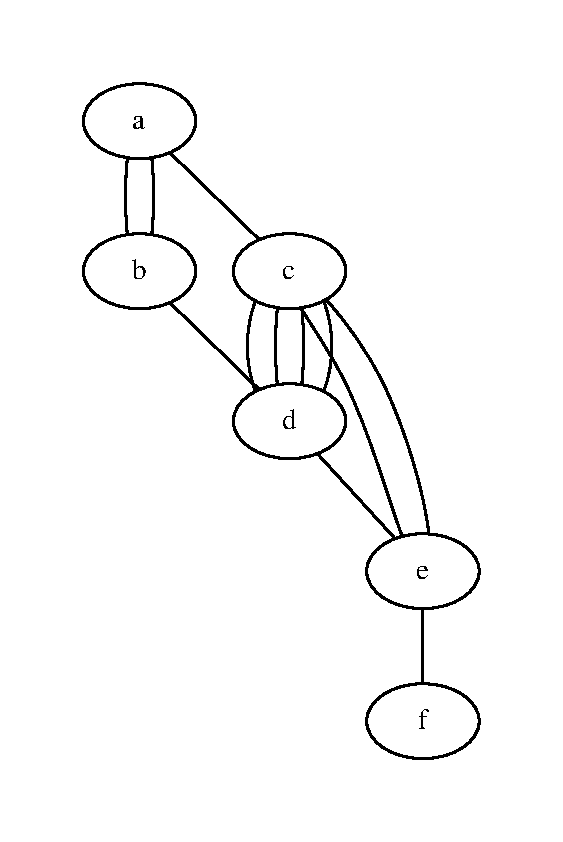
\includegraphics[scale=0.5]{multiple.pdf}
        \label{fig:exemplo-grafo-multiplo}
    }    
    \caption{Redes com laços e conexões múltiplas}
    \source{Elaboração do autor}
\end{figure}

Em algumas redes, não há sentido em nós que conectam a si mesmos, por exemplo, em uma rede social onde as conexões representam quem conhece quem, uma conexão de alguém consigo mesmo não é relevante para o estudo da rede (desconsiderando-se questões filosóficas). Já em outras redes é natural considerar esse tipo de conexão, como uma que modele a transição de estados de uma máquina em que uma ação pode resultar na permanência no mesmo estado. Conexões de um nó com ele mesmo são chamados \textit{laços} ou \textit{loops} (Figura~\ref{fig:exemplo-grafo-laco}).

Redes que não permitem laços, pesos ou múltiplas conexões entre dois nós são chamadas \textit{redes simples} (Figura~\ref{fig:exemplo-grafo-simples}).

% Ronie: Mover o parágrafo abaixo para a seção do Mapa de Carreiras?
Nessa pesquisa, o problema foi modelado como uma rede direcionada, ponderada e com laços. Cada ocupação é um nó, a movimentação de profissionais entre as ocupações são conexões direcionadas e ponderadas e os profissionais que permanecem na mesma ocupação mas mudam de empresa são modelados como laços.

O conceito de \textit{componente} é importante para esse trabalho e está relacionado a partes da rede que estão desconectadas entre si. Se existirem nós em uma rede que estão conectados entre si, mas não se conectam a nenhum outro nó, então essa rede \enquote{isolada} é um componente. Um nó sem conexões pode ser considerado um componente de tamanho~1. Uma rede em que todos os nós se conectam de maneira direta ou indireta é chamada de \textit{rede conectada} e possui apenas um componente. Um componente é um subgrafo em que todos os seus nós possuem conexão direta ou indireta entre si, porém nenhum de seus nós se conecta ao resto da rede. Uma exemplo de rede com três componentes pode ser observado na Figura~\ref{fig:exemplo-componente}.

\begin{figure}[ht]
    \centering
    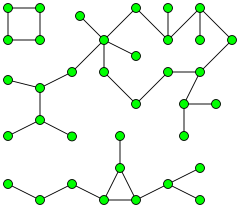
\includegraphics[scale=0.7]{componente.png}
    \caption{Rede com três componentes}
    \source{Wikimedia - David Eppstein}
    \label{fig:exemplo-componente}
\end{figure}

Em algumas topologias de rede surgem nós com um número de conexões muito acima do esperado, chamados \textit{hubs}. O número de conexões de um nó é chamado de \textit{grau} do nó, portanto, \textit{hubs} são nós de alto grau. Esse é um conceito central no estudo de redes complexas por não aparecerem em redes aleatórias, mas figurarem em diversas redes reais.

No estudo de redes, os nós de maior importância são considerados nós centrais da rede. Como é responsabilidade de cada estudo definir o que é \textit{importante}, existem várias medidas de centralidade, indo desde a simples contagem de nós com mais conexões (centralidade de grau) até a medição de nós que participam de fluxos de maior volume.


(EXPANDIR) Centralidade e Centralidade de Fluxo.

A medida de \textit{Assortatividade} significa que nós que compartilham características comuns tendem a se conectar com mais frequência. \textit{Desassortatividade} é o conceito contrário, onde nós com características diferentes tendem a se conectar mais frequentemente. Na Ciência de Redes é comum o termo ser associado a tendência de nós de mesmo grau se conectarem entre si. A assortatividade é detalhada na Seção~\ref{sec:assortatividade}. A grosso modo, uma assortatividade de grau negativa significa que a topologia da rede se assemelha à estrutura de \enquote{centro e raios\footnote{Em inglês: \enquote{Hub and Spokes}}}. Esse medida é importante na caracterização das ilhas ocupacionais.

(EXPANDIR) Bigramas e Trigramas

(EXPANDIR) Source e Sink

%====================================
\subsubsection{Redes Multicamadas} \label{sec:multicamadas}

Redes reais nem sempre podem ser modeladas como redes simples. Múltiplos tipos de relacionamentos como comunicação por email, telefone e pessoalmente; diferentes tipos de nós, como humanos e máquinas ou ainda diferentes momentos de interação, como conversas em um evento, bar ou no trabalho são características importantes que não são facilmente modeladas por redes tradicionais~\cite{Kivela2014-pb}.

Ao longo das últimas décadas, variações de modelos de rede foram utilizadas para modelar esses fenômenos, como redes multiplexadas, redes multirrelacionais e \enquote{redes de redes}. Em seu trabalho, \citeonline{Kivela2014-pb} propõem uma padronização dessas definições ao redor do termo Redes Multicamadas.

Uma rede multicamada representa a diversidade de nós e conexões acima exemplificados como uma rede em os nós possuem múltiplas representações, cada uma em uma \textit{camada} diferente. Um exemplo de rede multicamada pode ser visto na Figura~\ref{fig:ex-multicamada}.

\begin{figure}[ht]
    \centering
    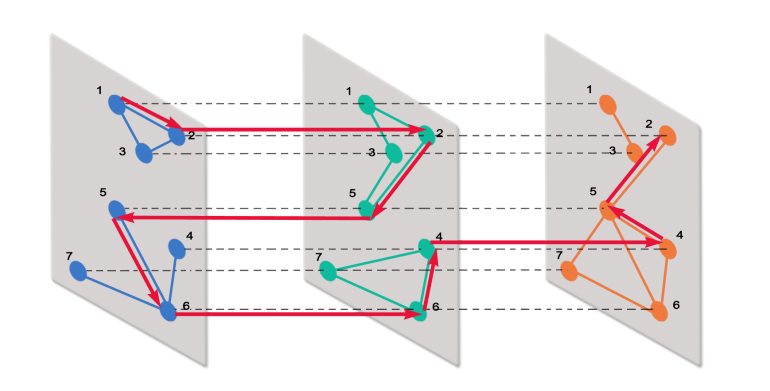
\includegraphics[scale=0.4]{random_walks_on_multilayer_networks}
    \caption{Exemplo do caminhar de um \textit{random walker} em uma rede multicamada.}
    \source{Wikimedia - Manlio De Domenico}
    \label{fig:ex-multicamada}
\end{figure}

Nessa trabalho, a rede multicamada é usada para simplificar uma rede modelada como um processo de Markov de segundo nível. Essa simplificação permite traduzir a Equação de Mapa (apresentada mais à frente, na Seção~\ref{sec:infomap}) para detectar sobreposições entre comunidades, ou seja, comunidades que compartilham nós.

%====================================
\subsection{Medidas de Rede} \label{sec:medidas-de-rede}

As medidas descritas nessa seção são usadas para caracterização da rede do MCar bem como das ilhas ocupacionais encontradas.

Entenda-se por \textit{caracterização} a descrição da rede utilizando medidas numéricas que permita a interpretação dos macro-atributos da rede. Por exemplo, a medida de assortatividade é usada para identificar que a topologia predominante nas ilhas ocupacionais se assemelha a de \textit{centro e raios}, enquanto a medida de centralidade de fluxo e de grau é usada para identificar as ocupações mais importantes nas ilhas.

%===================================
\subsubsection{Assortatividade} \label{sec:assortatividade}

A assortatividade é uma medida de quão nós similares estão conectados entre si~\cite{Newman2003-jn}. Quaisquer atributos dos nós podem ser usados como medida de assortatividade, por exemplo, se nós representarem pessoas e as conexões representarem amizades, medir a assortatividade de idade diria se as pessoas preferem amizades com outras de idade similar (assortatividade positiva) ou preferem amizades com pessoas muito mais velhas ou novas (assortatividade negativa ou desassortatividade).

A assortatividade de grau é de especial interesse na análise de redes, pois permite caracterizar sua topologia. Redes com assortatividade negativa (desassortativas), remetem à topologia de \textit{eixo e raios} ou \textit{estrela}, onde nós de grau muito alto (\textit{hubs}) se conectam a muitos nós de grau mais baixo~\cite{Barabasi2016-rn}. A Figura~\ref{fig:assortatividade-topologia} mostra um exemplo de uma rede em que predomina essa topologia.

Quanto menor a assortatividade, mais a rede se aproxima da topologia de estrela, em que todos os nós de alto grau conectam-se somente a nós de grau muito baixo. Como exemplos, a ilha ocupacional relacionada a \enquote{Fonoaudiologia} na Figura~\ref{fig:ex-assortatividade-negativa}, com assortatividade $-0,99$, possui todos os nós conectados a um \textit{hub} central, com nenhuma conexão entre as ocupações periféricas. Já a ilha relacionada a \enquote{Coordenador de Mídia} na Figura~\ref{fig:ex-assortatividade-positiva}, com assortatividade $0,18$, possui uma estrutura um pouco mais distribuída e o grau dos nós é similar, com exceção do próprio \enquote{Coordenador de Mídia}.

\begin{figure}[ht]
    \centering
    \subfloat[][Assortatividade $-0,99$] {
        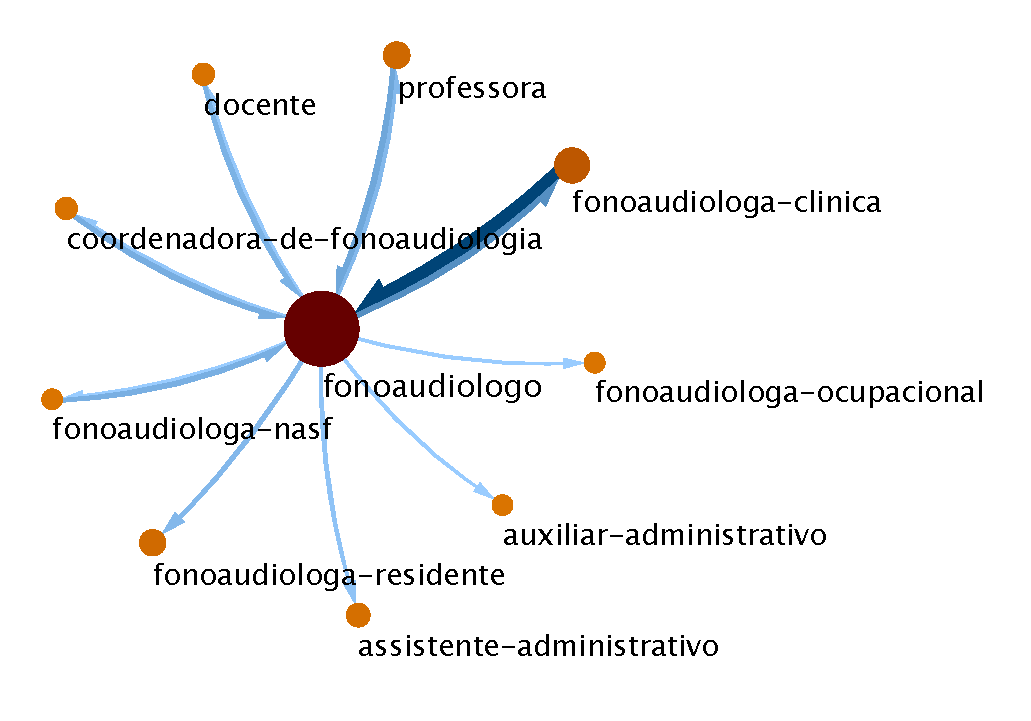
\includegraphics[width=0.4\linewidth]{ex-assortatividade-negativa.pdf}
        \label{fig:ex-assortatividade-negativa}
    }
    \subfloat[][Assortatividade $0,18$] {
        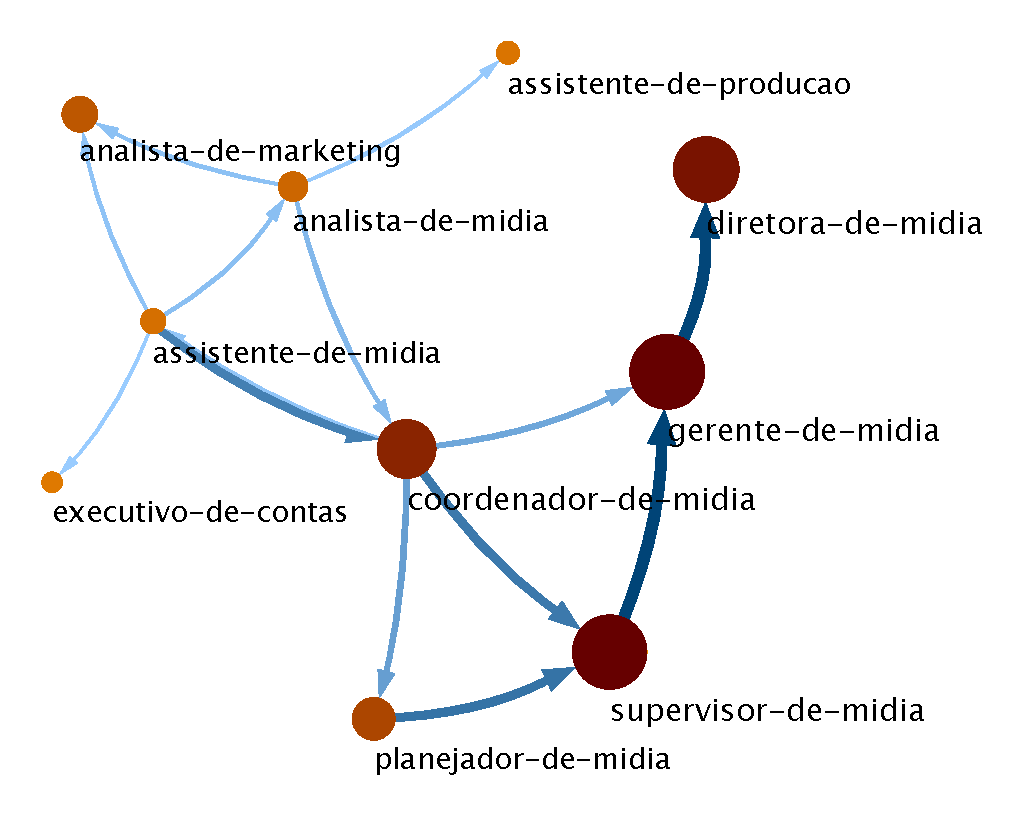
\includegraphics[width=0.4\linewidth]{ex-assortatividade-positiva.pdf}
        \label{fig:ex-assortatividade-positiva}
    }    
    \caption{Assortatividade e Topologia}
    \label{fig:assortatividade-topologia}
\end{figure}

A assortatividade de grau em uma rede direcionada pode ser caracterizada pelo coeficiente de correlação de Pearson dos graus~\cite{Barabasi2016-rn}. Seja $k_i^\leftarrow$ e $k_i^\rightarrow$,  respectivamente, os graus de entrada e saída do nó $i$, seja $E$ o conjunto de conexões da rede, $e = (m, n) \mid e \in E$ as conexões de $E$, $m$ o vértice de onde $e$ sai e $n$ o vértice para onde $e$ aponta, definem-se os \textit{graus remanescentes} de entrada e saída, respectivamente, $\delta_e^\leftarrow$ e $\delta_e^\rightarrow$ da conexão $e$ como
\begin{align*}
\delta_e^\leftarrow &= k_n^\leftarrow - 1
\\
\delta_e^\rightarrow &= k_m^\rightarrow - 1\,.
\end{align*}

\begin{figure}[ht]
    \centering
    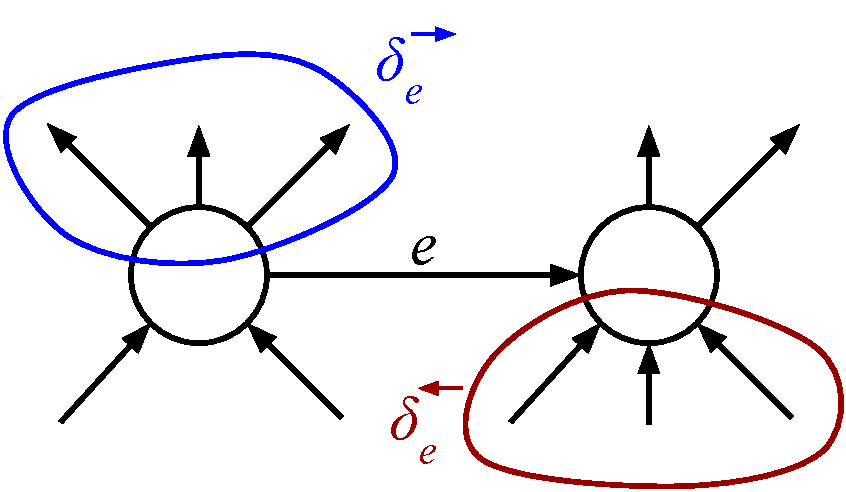
\includegraphics[scale=0.4]{remaining-degree.pdf}
    \caption{Graus remanescentes de entrada e saída da conexão $e$}
    \label{fig:remaining-degree}
\end{figure}

O \textit{grau remanescente} é o grau do nó, excetuando-se a conexão atual (Figura~\ref{fig:remaining-degree}). A correlação de Pearson $r$ dos graus é então definida por

\begin{align*}
p &= \sum_{e \in E} \delta_e^\leftarrow \delta_e^\rightarrow
\\
q &= \frac{1}{|E|} \sum_{e \in E} \delta_e^\leftarrow
\sum_{e \in E }\delta_e^\rightarrow
\\
\sigma^2_\leftarrow &= \sum_{e \in E} \left( \delta_e^\leftarrow \right)^2
- \frac{1}{|E|} \left( \sum_{e \in E} \delta_e^\leftarrow \right)^2
\\
\sigma^2_\rightarrow &= \sum_{e \in E} \left( \delta_e^\rightarrow \right)^2
- \frac{1}{|E|} \left( \sum_{e \in E} \delta_e^\rightarrow \right)^2
\\
r &= \frac{p - q}
{\sqrt{ \sigma^2_\leftarrow } \sqrt{ \sigma^2_\rightarrow }}\,.
\end{align*}

%====================================
\subsubsection{Coeficiente de Agrupamento} \label{sec:coeficiente-agrupamento}

O \textit{coeficiente de agrupamento local} é a medida de quanto os vizinhos de um nó estão conectados entre si e é dado por:

\begin{equation}
c_c(i) \defn \begin{cases}
    \frac{2m_i}{k_i(k_i - 1)} & \text{se}\ k_i > 1 \\
    \text{indefinido}         & \text{caso contrário}
  \end{cases}
\end{equation}

Onde $m_i$ é o número de conexões entre os vizinhos do nó $i$, e $k_i$ é o número de conexões de $i$.

O coeficiente de agrupamento local pode ser estendido para grafos direcionados distinguindo-se a direção da conexão.

\begin{equation}
\linkboth{c}_c(i) \defn \begin{cases}
    \frac{\linkboth{m}_i}{k_i(k_i - 1)} & \text{se}\ k_i > 1 \\
    \text{indefinido}                  & \text{caso contrário}
  \end{cases}
\end{equation}

Onde $\linkboth{m}_i$ é o número de conexões entre os vizinhos de $i$.

Em um grafo ponderado, \citeonline{Barrat2004-xf} oferecem a seguinte versão do coeficiente de agrupamento:

\begin{equation}
\weighted{c}_c(i) \defn \frac{1}{s_i(k_i - 1)} \sum_{j,k \in N(i)} \frac{w_{ij} + w_{jk}}{2}
\end{equation}

Onde $N(i)$ é o conjunto de vizinhos de $i$, $w_{ij}$ é o peso da conexão entre os nós $i$ e $j$ e $s(i)$ é a força do nó.

O \textit{coeficiente de agrupamento global} de um grafo é dado pela média dos coeficientes locais:

\begin{equation}
C_c \defn \frac{1}{|N'|} \sum_{i \in N'} c_c(i)
\end{equation}

Onde $N'$ é o conjunto de nós com grau maior que 1, ou seja, $N' = \left\lbrace i \in N \mid k_i > 1 \right\rbrace$. O coeficiente de agrupamento para um grafo ponderado é calculado da mesma forma, apenas substituindo-se o coeficiente local por sua versão ponderada.

\begin{comment}
%====================================
\subsubsection{Similaridade} \label{sec:similaridade}

A \textit{similaridade} é usada para medir se dois nós ou conexões são similares estruturalmente, ou seja, independente do seu conteúdo. De maneira simplificada, dois nós são tão mais similares quanto houverem vizinhos comuns. Já a \textit{similaridade de conexão}, como definida por \citeonline{Ahn2010-uh}, parte de conexões que compartilham um nó e verifica se os nós não compartilhados são similares.

A similaridade também é usada como medida de distância em algoritmos de agrupamento hierárquico \cite{Barabasi2016-rn}.

Existem diversas formulações para a similaridade e \citeonline{Lu2011-og} revisam dez delas sem considerar suas variações para redes direcionadas e ponderadas. Esse trabalho utiliza a similaridade baseada no índice de Jaccard (Equação~\ref{eq:similaridade-1}) e suas variações.

Sejam $i$ e $j$ nós da rede, $N_i$ o conjunto de vizinhos do nó $i$ e $N_i^+ \defn N_i \cup \{i\}$, a Equação~\ref{eq:similaridade-1} define a similaridade por vizinhança e a Equação~\ref{eq:similaridade-2} define a mesma similaridade considerando a existência de conexão direta entre os nós sendo comparados.

\noindent
\begin{tabularx}{\linewidth}{@{}XX@{}}
    \begin{equation} \label{eq:similaridade-1}
        S_{ij} \defn \frac{|N_i \cap N_j|}{|N_i \cup N_j|} 
    \end{equation} &
    \begin{equation} \label{eq:similaridade-2}
        S_{ij}^+ \defn \frac{|N_i^+ \cap N_j^+|}{|N_i^+ \cup N_j^+|} 
    \end{equation}
\end{tabularx}

Em redes direcionadas é preciso distinguir os vizinhos de entrada e saída. A similaridade em uma rede direcionada $\linkboth{S}_{ij}$ é dada pela média entre similaridade de entrada e saída (Equação~\ref{eq:similaridade-3}).

\begin{equation} \label{eq:similaridade-3}
    \linkboth{S}_{ij} \defn \frac{1}{2} \left( \frac{|\linkin{N}_i \cap \linkin{N}_j|}{|\linkin{N}_i \cup \linkin{N}_j|} + \frac{|\linkout{N}_i \cap \linkout{N}_j|}{|\linkout{N}_i \cup \linkout{N}_j|} \right)
\end{equation}

Onde $\linkin{N}_i$ é o número vizinhos de $i$ em que as conexões chegam a ele e $\linkout{N}_i$ é o número de vizinhos onde a conexão parte de $i$.

No caso de redes ponderadas e direcionadas, o índice de Jaccard pode ser generalizado no coeficiente de Tanimoto, resultando na similaridade $\weighteddir{S}_{ij}$ da Equação~\ref{eq:similaridade-3} \cite{Ahn2010-uh}. Sendo $W$ a matriz de pesos da rede e $w_{ij}$ o peso da conexão direcionada de $i$ a $j$, define-se o vetor $\vec{w}_i = (w_{i1},w_{i2},\ldots,w_{in})$ como sendo o vetor de pesos das conexões do nó $i$, onde $n$ é o número de nós da rede e $w_{ij} = 0$ se não há conexão entre os nós.

\begin{equation}
\weighteddir{S}_{ij} \defn \frac{\vec{w_i} \cdot \vec{w_j}}{|\vec{w_i}|^2 + |\vec{w_j}|^2 - \vec{w_i} \cdot \vec{w_j}}
\end{equation}

Para o agrupamento de conexões, como proposto por \citeonline{Evans2009-lq} e \citeonline{Ahn2010-uh}, é preciso definir a similaridade entre conexões. Sendo o vetor $\vec{r}_{i} \defn (r_{i1}, r_{i2}, \ldots, r_{iN})$ definido de acordo com a Equação~\ref{eq:similaridade-conexao-parcial}:

\begin{equation} \label{eq:similaridade-conexao-parcial}
r_{ij} \defn \frac{1}{k_i} \sum_{h \in N_i} w_{ih}\delta_{ij} + w_{ij}
\end{equation}

Onde $\delta_{ij} = 1$ se $i = j$ e zero caso contrário. A similaridade entre conexões $R_{(i,h),(h,j)}$ pode ser definida como \cite{Ahn2010-uh}:

\begin{equation}
R_{(i,h),(j,h)} \defn \frac{\vec{r_i} \cdot \vec{r_j}}{|\vec{r_i}|^2 + |\vec{r_j}|^2 -  \vec{r_i} \cdot \vec{r_j}}
\end{equation}

Onde $(i,h)$ e $(j,h)$ são as conexões que compartilham o nó $h$ e $i \neq h \neq j$. O nó compartilhado não é usado no cálculo da similaridade, mas é pré-requisito para considerar que duas conexões são similares. A similaridade de conexão é usada principalmente na detecção de comunidades.
\end{comment}

%====================================
\subsubsection{Modularidade} \label{sec:modularidade}

A \textit{modularidade} é uma medida de qualidade para a detecção de comunidades. O algoritmo de Louvain, por exemplo, usa a modularidade como função objetivo~\cite{Barabasi2016-rn}. De certa forma ela tem uma relação com o coeficiente de agrupamento, no sentido que ambas procuram quantificar o quanto nós estão mais densamente conectados que outros.

Essa medida é aplicada apenas a um grafo que foi particionado em comunidades. Em termos gerais, ela fornece um indício se um grupo de nós é mais densamente conectado que o esperado em um modelo nulo, em caso afirmativo, esse conjunto é uma possível comunidade. Para o caso em que ela reflete um comportamento próximo do que seria esperado em uma rede aleatória, não é possível afirmar que esse grupo tenha qualquer característica especial que o transforme em uma comunidade. No caso de modularidade negativa, isto é, em que a densidade de conexões é menor do que o esperado, esse grupo não representa uma comunidade~\cite{Barabasi2016-rn}.

A modularidade $m_c$ de um grupo $c$ de nós pode ser definida como:

\begin{equation} \label{eq:modularidade-local}
m_c \defn \frac{L_c}{L} - \left( \frac{K_c}{K} \right)^2
\end{equation}

Onde $L$ é o número total de conexões da rede, $K = 2L$ é a soma de todos os seus graus, $L_c$ é o número de conexões do grupo e $K_c$ é a soma de seus graus.

Assumindo que uma rede foi particionada em $N_c$ grupos, a modularidade total $M_c$ pode ser calculada somando-se a modularidade de cada grupo:

\begin{equation} \label{eq:modularidade-global}
M_c \defn \sum_{c \in N_c} m_c
\end{equation}

O uso da modularidade para detecção de comunidades possui limitações. A primeira delas é que grupos com poucas conexões internas em relação ao tamanho da rede são agrupados indevidamente, mesmo que exista apenas uma conexão entre eles. A segunda limitação diz respeito ao maior valor possível da modularidade $M_\textit{max}$, que possui a tendência de formar um platô, dificultando a detecção da partição ótima~\cite{Barabasi2016-rn}.

Considerando as Equações \ref{eq:modularidade-local} e \ref{eq:modularidade-global}, quando dois grupos $A$ e $B$ são unidos, a diferença esperada em $M_c$ é:

\begin{equation}
\Delta M_{AB} \defn \frac{l_{AB}}{L} - \frac{k_A k_B}{2L^2}
\end{equation}

Onde $l_{AB}$ é o número de conexões que conectam os dois grupos, e $k_A$ e $k_B$ são as somas de graus de $A$ e $B$, respectivamente. Quando $k_A k_B / 2L^2 < 1$, a modularidade aumenta ($\Delta M_{AB} > 0$) se houver ao menos uma conexão entre os grupos ($l_{AB} \geq 1$). Isso significa que esses grupos unidos aumentam a modularidade, mesmo sendo grupos diferentes. Esse efeito é chamado de \textit{resolução da modularidade}.

É possível observar que a resolução da modularidade é diretamente proporcional ao número total de conexões da rede. Diminuindo-se o número de conexões, $k_A$ e $k_B$ se tornam mais relevantes que $l_{AB} / L$. Portanto, para contornar essa limitação é possível considerar os maiores grupos da partição como uma única rede e reparticioná-la. Dessa forma, os grupos artificialmente unidos por conta da resolução serão separados.

\todo[inline]{Demonstrar separando a carreira de TI aqui}


%====================================
\subsection{Detecção de Comunidade} \label{sec:deteccao-comunidade}

Detecção de Comunidade, Particionamento de Grafo, Agrupamento (\textit{Clustering}) ou Modelagem de Bloco (\textit{Block Modelling}) são nomes equivalentes para a atividade de se encontrar conjuntos de nós que possuem ligações mais fortes entre si do que com o resto da rede.

\citeonline{Barabasi2016-rn} propõem quatro hipótese sobre detecção de comunidade.

\begin{description}
%--------------------------------
\item [Hipótese Fundamental] \textit{A estrutura de comunidade de uma rede é codificada unicamente em seu diagrama de conexões.}

Isso significa que não é possível identificar comunidades somente pelos seus graus, nós ou quaisquer medidas que não envolvam a estrutura de conexão da rede. A detecção de comunidades só é possível analisando-se a conectividade entre os nós, seja através de uma matriz de adjacência ou outro artefato que permita a investigação das conexões.

%--------------------------------
\item [Hipótese da Conectividade e Densidade] \textit{Uma comunidade é um subgrafo densamente conectado em uma rede.}

\textit{Conectividade} significa que uma comunidade não ultrapassa as bordas de um único componente, já \textit{Densidade} significa que os membros de uma comunidade têm maior probabilidade de se conectarem entre si do que com membros fora dela.

%--------------------------------
\item [Hipótese de Aleatoriedade] \textit{Redes aleatoriamente conectadas não possuem estrutura de comunidade}

Essa hipótese é um dos fundamentos para a medida de Modularidade descrita na Seção~\ref{sec:modularidade}, embora tenha sido formalmente postulada após a concepção da medida por \citeonline{Newman2004-by}. De acordo com essa hipótese, uma comunidade é um conjunto de nós mais fortemente conectado do que o esperado em um modelo nulo equivalente. Essa definição está de acordo com a premissa de um modelo nulo que, se uma estrutura pode emergir por pura aleatoriedade, então não pode ser atribuída a ela um princípio de organização vindo de outra fonte.

%--------------------------------
\item [Hipótese de Modularidade Máxima] \textit{Para uma dada rede, a partição com modularidade máxima corresponde à estrutura ótima da comunidade.}

Essa hipótese se baseia na anterior, justificando que quanto mais longe a estrutura de uma comunidade estiver de uma estrutura aleatória, mais relevante ela é como comunidade. Entretanto, como discutido na Seção~\ref{sec:modularidade}, essa definição possui limitações quanto ao seu uso prático por conta dos problemas de \textit{resolução} e \textit{platô}.

\end{description}

%===================================
\subsection{Equação de Mapa} \label{sec:infomap}
%===================================

Segundo \citeonline{Grunwald2007-bt}, quaisquer regularidades em um conjunto de dados podem ser usadas para comprimi-lo, ou seja, descrevê-lo usando uma quantidade menor de símbolos. Quanto maior a regularidade, maior a compressão, dessa forma, dentre várias representações possíveis dos dados, a que apresentar maior compressão é também aquela que melhor identifica padrões nos dados. A Descrição de Comprimento Mínimo (\textit{Minimum Description Length}) é a disciplina que estuda essa relação~\cite{Grunwald2007-bt}.

O algoritmo Infomap aproveita essa dualidade entre detecção de padrões e compressão de dados para identificar padrões de fluxo em redes~\cite{Rosvall2009-sd}.

Para compreender o algoritmo, é preciso entender como um trajeto aleatório em uma rede é representado e como a Descrição de Comprimento Mínimo usa essa representação na detecção de comunidades.

Para isso, descreve-se o caminho que um \textit{random walker} faz em uma rede através da sequência de nós pela qual ele passa. Por exemplo, assumindo uma rede com os nós $A$, $B$ e $C$, um caminho possível poderia ser descrito por $ABACBA$.

A Figura~\ref{fig:graph01} mostra um grafo regular, onde todos os nós possuem três vizinhos. Nesse tipo de rede, um \textit{random walker} ergódico (de caminho infinito) percorre todas as conexões o mesmo número de vezes. A Figura~\ref{fig:walk01} mostra um caminho aleatório passando por 800 nós.

\begin{figure}[ht]
    \centering
    \subfloat[][Rede regular] {
        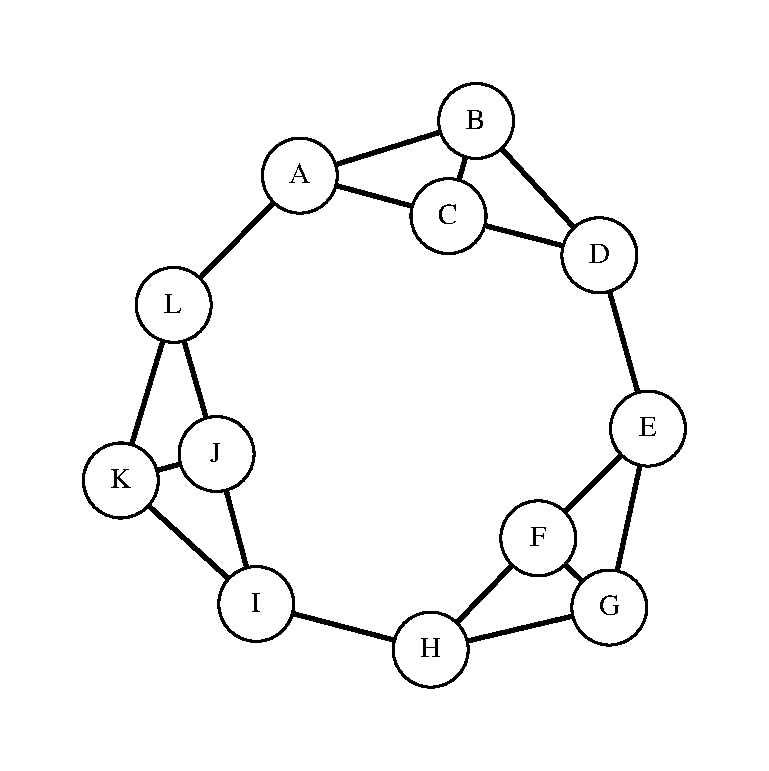
\includegraphics[scale=0.4]{graph01.pdf}
        \label{fig:graph01}
    }
    \subfloat[][Caminho na rede] {
        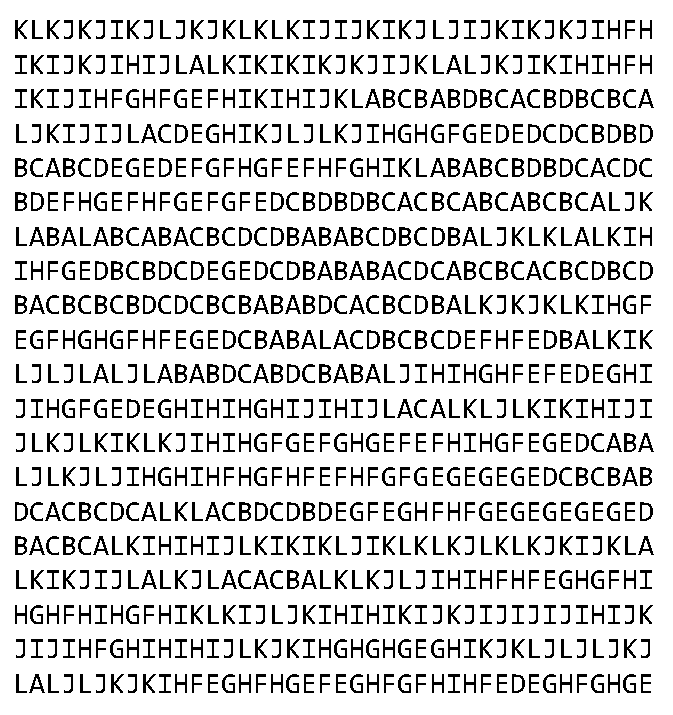
\includegraphics[scale=0.4]{graph01_path.pdf}
        \label{fig:walk01}
    }    
    \caption{Caminho de um \textit{random walker}}
\end{figure}

Apesar de ser uma rede regular, onde cada nó possui três conexões, sua topologia faz com que o \textit{random walker} fique \enquote{preso} nos grupos formados pelos nós $ABCD$, $EFGH$ e $IJKL$; escapando esporadicamente de um para outro, onde circula até escapar novamente. Esses grupos são destacados na Figura~\ref{fig:graph02}. O caminho percorrido pelo \textit{walker} é exibido na Figura~\ref{fig:walk02}, dessa vez destacando os grupos por onde ele passa. As cores em ambas as figuras tornam fácil perceber seu comportamento.

\begin{figure}[ht]
    \centering
    \subfloat[][Rede regular] {
        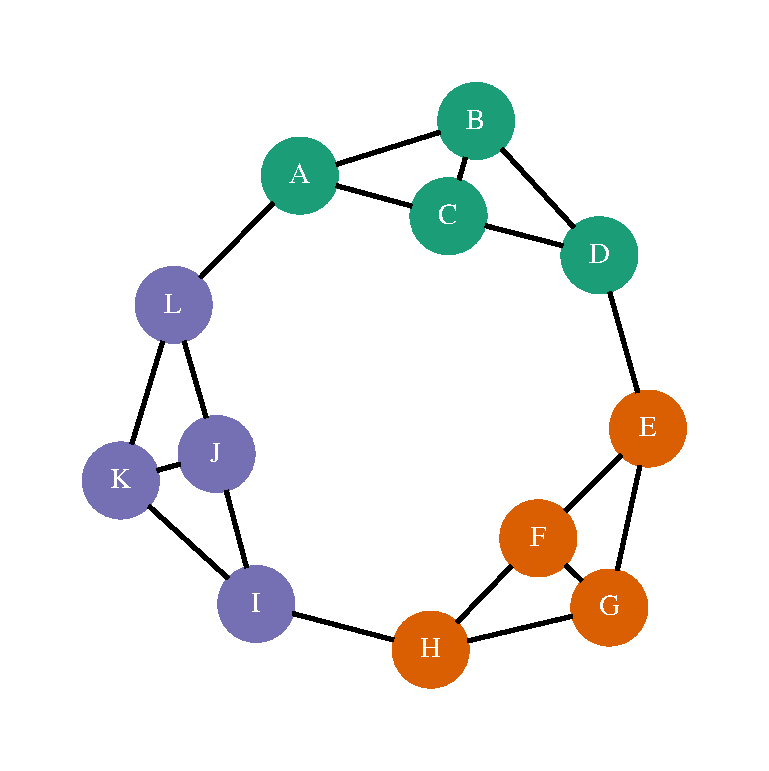
\includegraphics[width=0.4\linewidth]{graph02.pdf}
        \label{fig:graph02}
    }
    \subfloat[][Caminho na rede] {
        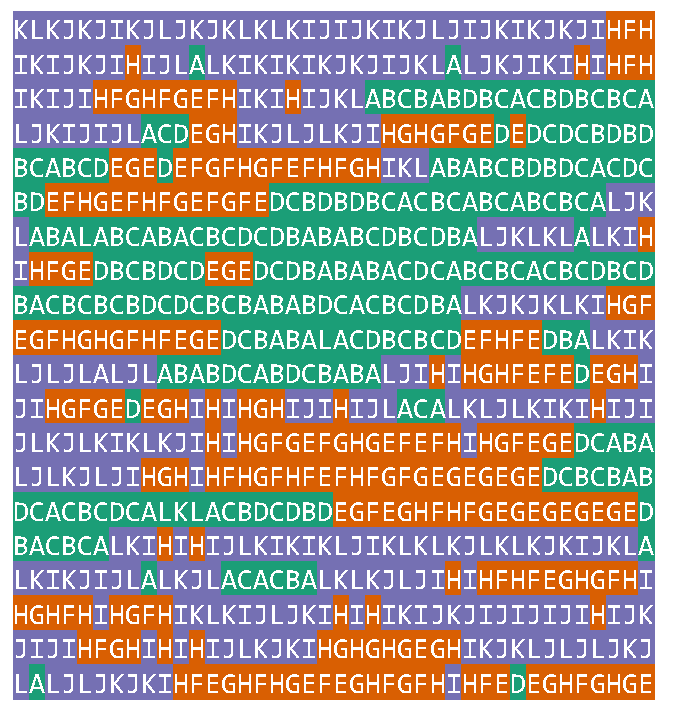
\includegraphics[width=0.4\linewidth]{graph02_path.pdf}
        \label{fig:walk02}
    }    
    \caption{Rede e caminho destacados}
\end{figure}

Se cada nó for representado por uma sequência de bits, podemos medir quanta informação é necessária para representar o caminho feito pelo \textit{random walker}. Usando a codificação de tamanho variável de  \citeonline{Huffman1952-ak} os nós mais frequentes são representados por códigos menores, o que leva a uma codificação menor para representar um caminho do que uma que use códigos de tamanho fixo.

Os códigos usados por cada grupo são chamados \textit{codebooks}, os códigos que indicam qual \textit{codebook} será usado também são \textit{codebooks}, funcionando como um índice. Na Figura~\ref{fig:graph04}, existem três deles, um para cada grupo, contendo os nós \enquote{00}, \enquote{01}, \enquote{10}, \enquote{110} e o código de saída \enquote{111}. O \textit{codebook} índice possui os códigos: \enquote{0}, \enquote{10} e \enquote{11}.

Dessa forma, sem o uso de \textit{codebooks}, o caminho que começa no nó mais abaixo do grafo da Figura~\ref{fig:graph03} e termina no nó do canto superior esquerdo é descrito pela sequência binária \enquote{000 1110 1011 1111 1101}, usando 19 bits. O mesmo caminho, usando a codificação com \textit{codebooks} da Figura~\ref{fig:graph04} é \enquote{\textbf{0} 01 110 \textit{111} \textbf{11} 00 01 10} e possui 17 bits (os números em negrito indicam entrada em um grupo e o número em itálico indica saída do grupo).

Nesse caminho curto, ambas as codificações têm tamanhos similares, porém, em um caminho infinitamente longo (ergódico), o uso de múltiplos \textit{codebooks} pode produzir um código mais compacto do que o uso de um único \textit{codebook}. Como exemplo, o caminho da Figura~\ref{fig:walk01} usando a codificação com um único \textit{codebook} da Figura~\ref{fig:graph03} possui 2880 bits contra 1776 bits usando a codificação com três \textit{codebooks} da Figura~\ref{fig:graph04}.

\begin{figure}[ht]
    \centering
    \subfloat[][Nós usando codificação de Huffman] {
        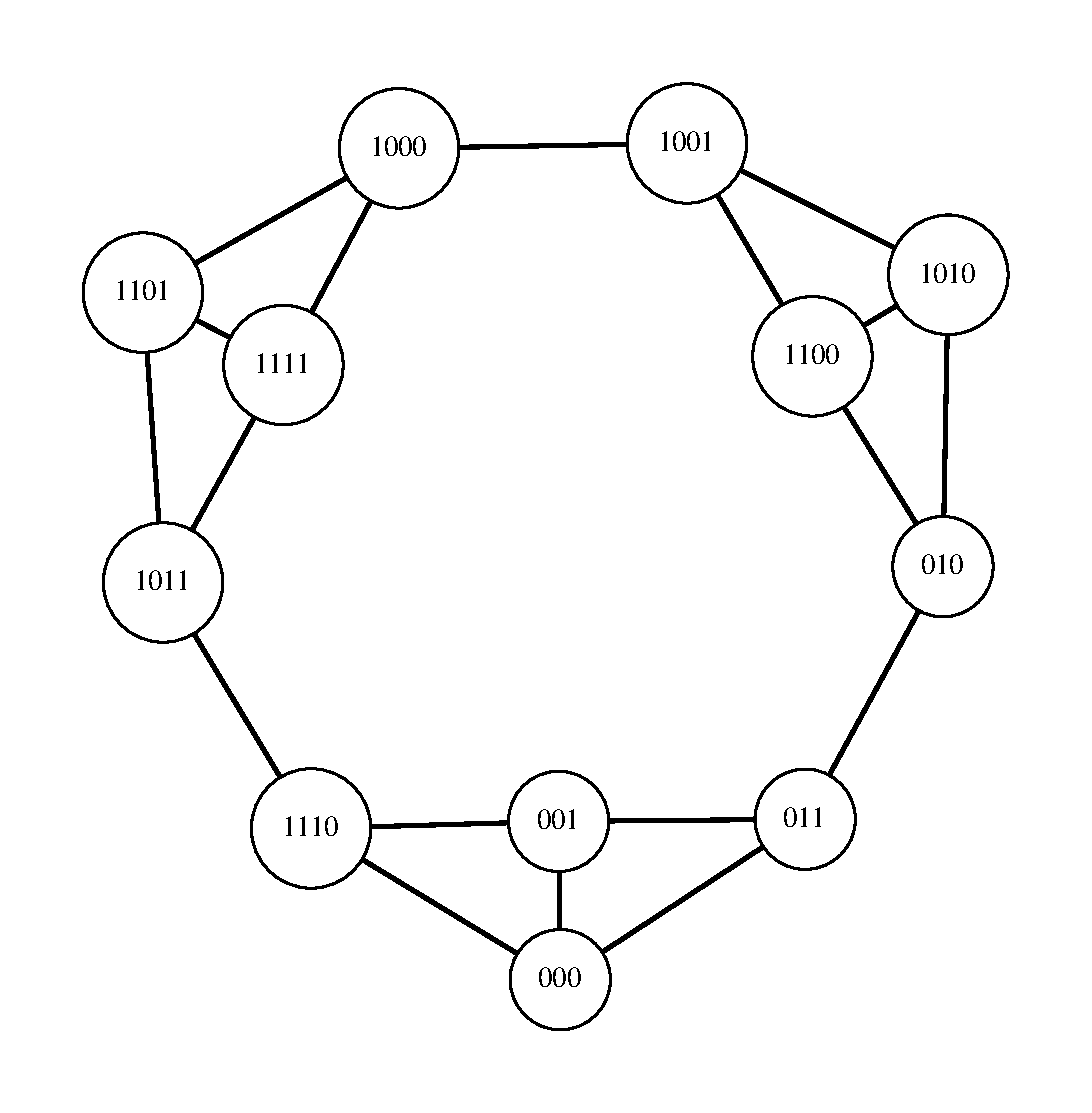
\includegraphics[width=0.4\linewidth]{graph03.pdf}
        \label{fig:graph03}
    }
    \subfloat[][Reaproveitamento de códigos] {
        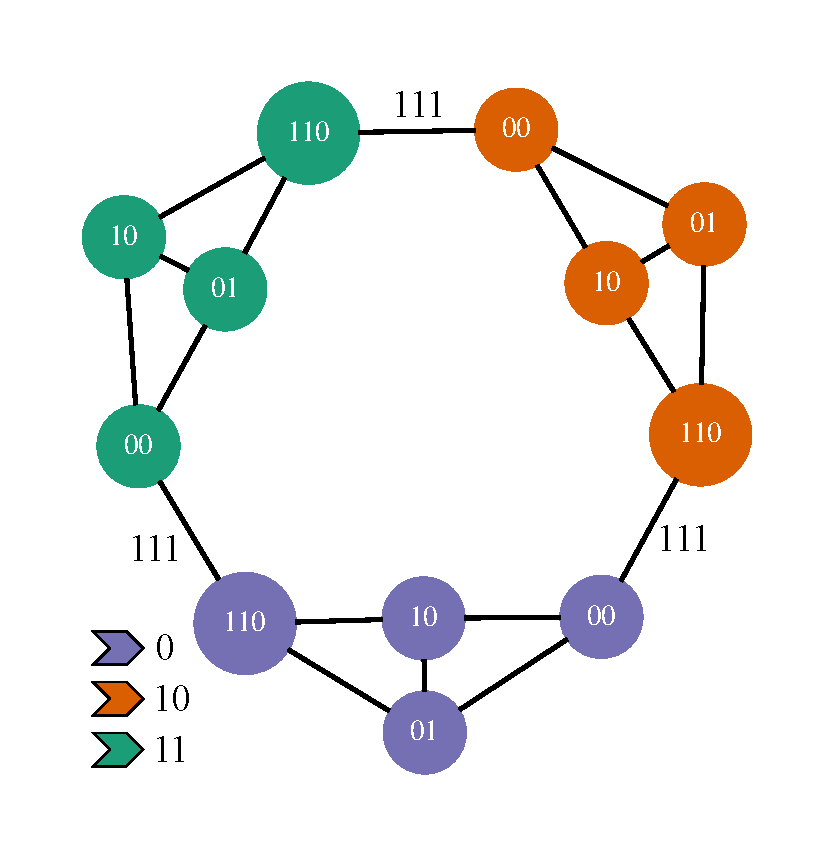
\includegraphics[width=0.4\linewidth]{graph04.pdf}
        \label{fig:graph04}
    }    
    \caption{Codificação dos nós}
\end{figure}

O particionamento da rede em grupos onde os caminhos aleatórios podem ser representados da maneira mais compacta possível deve representar o melhor particionamento em relação ao fluxo.

A \enquote{Equação de Mapa}\footnote{No original: \textit{Map Equation}}~\cite{Rosvall2009-sd} permite que se identifiquem as menores codificações possíveis para um determinado particionamento da rede sem a necessidade de se empregar \textit{random walkers} de fato. Com ela, a detecção de comunidades usando o fluxo como critério de coesão se reduz a um problema de otimização.

A Equação de Mapa é
\begin{equation} \label{eq:map-equation}
L(\mathsf{M}) = q_\curvearrowright H(\mathcal{Q}) + \sum_{i \in \mathsf{M}} p^i_\circlearrowright H(\mathcal{P}^i)\,,
\end{equation}
onde $L(\cdot)$ é o menor tamanho de codificação possível para representar um certo particionamento; $\mathsf{M}$ é o particionamento dos nós em comunidades $i \in \mathsf{M}$; $q_\curvearrowright$ é a probabilidade de um \textit{random walker} sair de qualquer comunidade e passar para o \textit{codebook} índice; $H(\mathcal{Q})$ (\textit{eta} em maiúsculo) é o número médio de bits usado para representar o \textit{codebook} índice segundo a distribuição de probabilidade $\mathcal{Q}$; e $H(\mathcal{P}^i)$ também é o número médio de bits, mas dessa vez daqueles usados na comunidade $i$ segundo a distribuição $\mathcal{P}^i$; finalmente $p^i_\circlearrowright$ é a probabilidade do \textit{walker} estar na comunidade $i$.

$H(\textbf{p})$ é a equação que descreve a entropia da informação segundo uma certa distribuição de probabilidade $\textbf{p}$~\cite{Shannon1948-ic}. Ela se refere a média de bits necessária, por símbolo, para se representar a informação gerada por um processo estocástico e é expressa como:
\begin{equation*}
H(\textbf{p}) = - \sum_\alpha p_\alpha \log_2 p_\alpha\,.
\end{equation*}

Nessa equação, $p_\alpha$ é a probabilidade estacionária da rede, ou seja, em um caminho infinito, qual fração de tempo o \textit{walker} estaria em $\alpha$~\cite{Rosvall2009-sd}.

Para calcular $p_\alpha$ inicia-se com a matriz estocástica linear $W$, gerada a partir da matriz de adjacência $A$ direcionada e ponderada. Em uma matriz estocástica linear, a soma dos pesos de entrada do nó (linha) é normalizada para que resulte em 1. Cada elemento $w_{\alpha \beta}$ dessa matriz representa a probabilidade de um \textit{random walker}  em $\alpha$ chegar ao nó $\beta$. Transportada para a realidade do MCar, essa é a probabilidade de alguém na ocupação $\alpha$ fazer a transição para a ocupação $\beta$.

Sendo $n$ o número de nós da rede, define-se $w_{\alpha \beta}$ como:
\begin{align} \label{eq:matriz-estocastica}
w_{\alpha \beta} = 
\begin{cases*}
\frac{1}{n}, & \text{se $\alpha$ não possui conexões de saída, ou seja, $\sum_\beta A_{\alpha \beta} = 0$,} \\
0, & \text{se não há conexão entre $\alpha$ e $\beta$,} \\
\frac{A_{\alpha \beta}}{\sum_\beta A_{\alpha \beta}}, & \text{caso contrário.}
\end{cases*}
\end{align}

A primeira cláusula da Equação~\ref{eq:matriz-estocastica} garante que a matriz estocástica possua linhas totalizando 1 quando o nó não possui conexões de saída. Para efeitos do \textit{random walker}, isso significa que ele se teleporta para um nó qualquer da rede quando se encontra em um nó sem saída. Caso contrário, os nós sem conexões de saída acumulariam a probabilidade total da rede~\cite{Page1999-ag}.

A probabilidade estacionária $p_\alpha$ é calculada pelo sistema de equações
\begin{equation} \label{eq:page-rank}
p_\alpha = \frac{1}{n} \tau + \sum_\beta (1 - \tau) p_\beta w_{\beta \alpha}\,,
\end{equation}
onde $\tau$ é a probabilidade do \textit{walker} ser teleportado para um nó aleatório. A primeira cláusula da Equação~\ref{eq:matriz-estocastica} e a presença de $\tau$ transformam o \textit{random walker} em um \textit{random surfer}. Esse artifício foi usado por~\citeonline{Page1999-ag} na criação do algoritmo de PageRank e fornece a base para a Equação de Mapa.

O recurso de teleporte garante a ergodicidade do caminho e, segundo o teorema de Perron-Frobenius, faz com que a probabilidade estacionária seja definida~\cite{Rosvall2009-sd}.

A partir de $p_\alpha$, é possível expandir a Equação de Mapa. Seja $q_{i \curvearrowright}$ a probabilidade de saída da comunidade $i$ e $q_{\curvearrowright}$ a probabilidade de saída de qualquer comunidade, o valor de $q_{\curvearrowright}$ equivale à taxa de uso do \textit{codebook} índice, uma vez que a saída de uma comunidade implica  em seu uso para indicar qual a próxima comunidade. Finalmente, seja $n$ o número de nós da rede e $n_i$ o número de nós pertencente à comunidade $i$, expande-se a Equação~\ref{eq:map-equation} em
\begin{align}
q_{i \curvearrowright} &= \frac{n - n_i}{n} \tau \sum_{\alpha \in i} p_\alpha + (1 - \tau) \sum_{\alpha \in i} \sum_{\beta \nin i} p_\alpha w_{\alpha \beta} \nonumber \\
q_\curvearrowright       &= \sum_{i \in M} q_{i\curvearrowright} \nonumber \\
p^i_\circlearrowright    &= q_{i \curvearrowright} + \sum_{\alpha \in i} p_\alpha \nonumber \\
H(\mathcal{Q})            &= - \sum_{i \in M} \frac{q_{i \curvearrowright}}{q_\curvearrowright} \log_2 \frac{q_{i \curvearrowright}}{q_\curvearrowright} \nonumber \\
H(\mathcal{P}^i)         &= - \frac{q_{i \curvearrowright}}{p^i_\circlearrowright} \log_2 \frac{q_{i \curvearrowright}}{p^i_\circlearrowright} 
-  \sum_{\alpha \in i} \frac{p_\alpha}{p^i_\circlearrowright} \log_2  \frac{p_\alpha}{p^i_\circlearrowright} \label{eq:eta-p} \\
L(\mathsf{M})              &= q_\curvearrowright \log_2 q_\curvearrowright - 2 \sum_{i = 1}^m q_{i \curvearrowright} \log_2 q_{i \curvearrowright} - \sum_{\alpha = 1}^n p_\alpha \log_2 p_\alpha + \sum_{i = 1}^m p^i_\circlearrowright \log_2 p^i_\circlearrowright\,. \nonumber
\end{align}

\subsection{Redes com Memória}  \label{sec:redes-com-memoria}

Na modelagem do MCar, um \enquote{Analista de Sistemas} e um \enquote{Arquiteto} têm chances similares de se tornarem \enquote{Coordenador de Projetos}. Entretanto, apesar de receber o mesmo nome, as competências de um coordenador de projetos da área de software e de arquitetura são bastante diferentes. Na realidade, essa é uma ocupação que pode figurar em duas ilhas ocupacionais bastante distintas, pois a movimentação entre essas duas áreas é relativamente rara em comparação com a movimentação dentro de si mesmas.

O padrão esperado nesse caso, é que profissionais de cada ilha vão para essa \enquote{Gerente de Projetos} e voltem para outras de sua própria ilha ao invés de cruzar a fronteira de carreira. Para poder identificar esse padrão, é preciso considerar não apenas o trabalho imediatamente anterior, mas também o subsequente.

No MCar as ocupações prévias do profissional não influenciam seu próximo passo, apenas sua ocupação atual. No entanto, como exemplificado no caso acima, a \enquote{perda de memória} da ocupação anterior compromete a identificação das comunidades.

Efetivamente, o MCar modela o fluxo de profissionais como um cadeia de Markov de primeira ordem. Considerar ocupações anteriores transforma o fluxo da rede em uma cadeia de Markov de ordem superior ou \enquote{Redes com Memória}\footnote{no original: \textit{Memory Networks}} \cite{Edler2017-kt}.

\begin{figure}[htb]
    \centering
    \subfloat[][Simples] {
        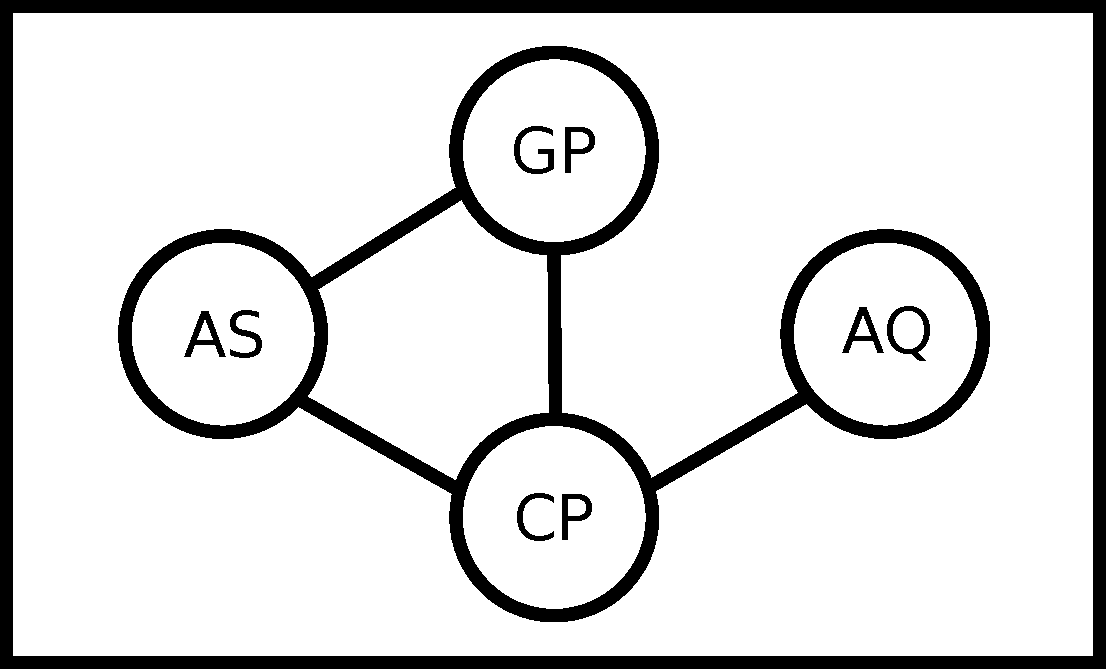
\includegraphics[width=0.3\linewidth]{ex-multilayer-04.pdf}
        \label{fig:ex-multilayer-simples}
    }
    \subfloat[][Direcionada]{
        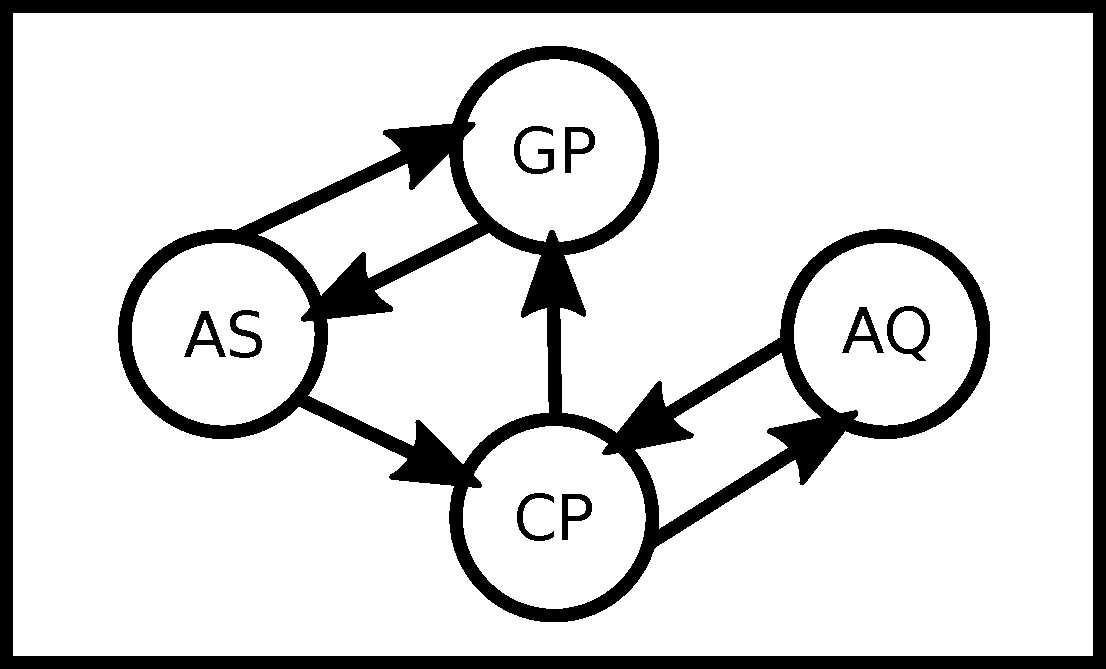
\includegraphics[width=0.3\linewidth]{ex-multilayer-05.pdf}
        \label{fig:ex-multilayer-direcionada}
    }
    \subfloat[][Trigramas] {
        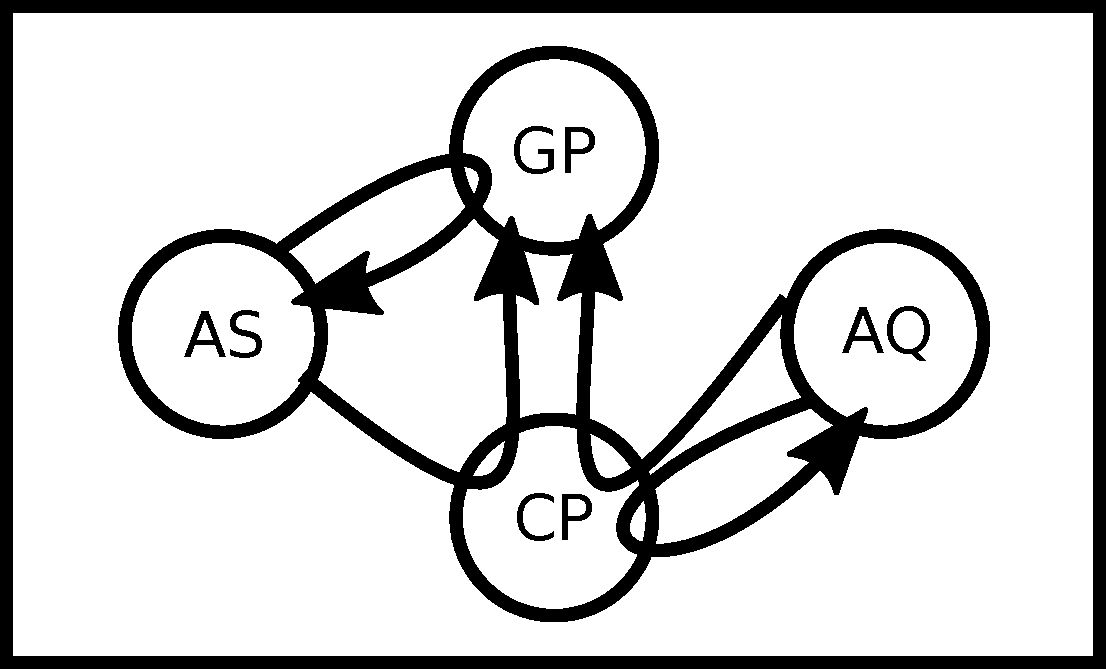
\includegraphics[width=0.3\linewidth]{ex-multilayer-01.pdf}
        \label{fig:ex-multilayer-trigrama}
    }
    \caption{Exemplo de uma rede com 4 nós e representações com sucessivos aumentos de informação. Os nós são GP - \textit{Gerente de Projetos}, AS - \textit{Analista de Sistemas}, AQ - \textit{Arquiteto} e CP - \textit{Coordenador de Projetos}. A rede simples da Figura~\ref{fig:ex-multilayer-simples} faz as conexões entre AS e CP agirem como bidirecionais; a rede direcionada da Figura~\ref{fig:ex-multilayer-direcionada} unifica as probabilidades de um \textit{random-walker} caminhar entre CP e GP, ignorando onde estava anteriormente. Os fluxos com dois níveis de memória (processo markoviano de segunda ordem) podem ser observados na Figura~\ref{fig:ex-multilayer-trigrama}}
\end{figure}

\citeonline{Edler2017-kt} adaptam a Equação de Mapa  para trabalhar com  Redes com Memória transformando-as em uma rede multi-camadas em uma representação chamada \enquote{Rede com Memória em Multi-Camadas}\footnote{no original: \textit{Multilayer Memory Network}}. Um rede multi-camadas é usada para representar redes em sistemas complexos onde existem contextos diferentes de relacionamento~\cite{Kivela2014-pb}. Por exemplo, em uma rede social onde pessoas participam de vários eventos, cada camada pode representar um evento, enquanto os relacionamentos podem representar a interação entre elas em cada evento. 

\begin{figure}[htb]
    \centering
    \subfloat[][Trigramas] {
        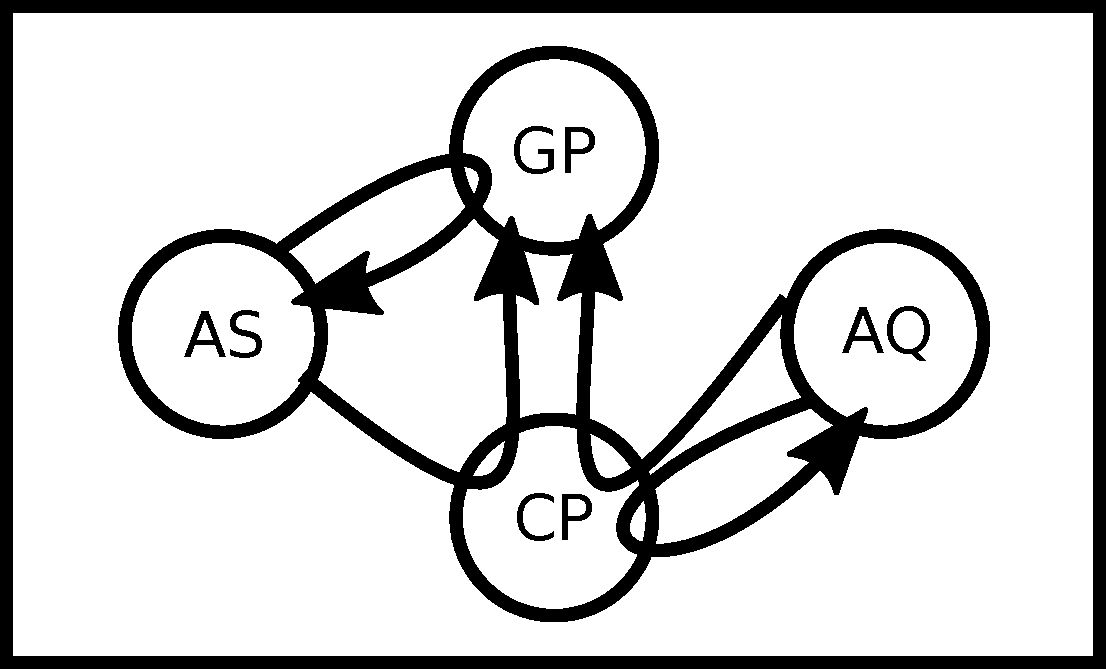
\includegraphics[width=0.3\linewidth]{ex-multilayer-01.pdf}
        \label{fig:ex-multilayer1}
    }
    \subfloat[][Como camadas] {
        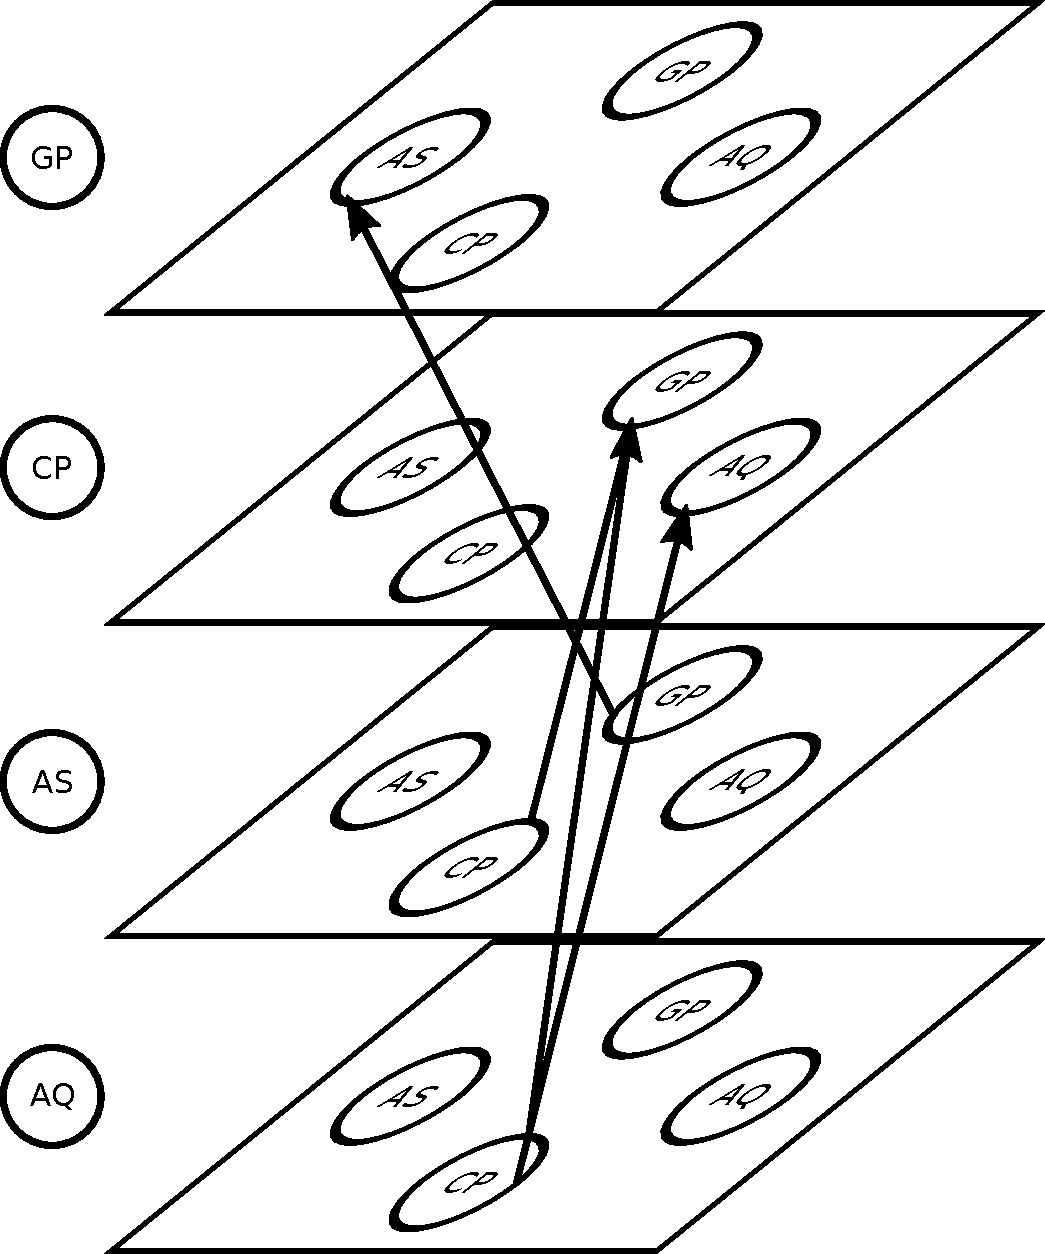
\includegraphics[width=0.3\linewidth]{ex-multilayer-02.pdf}
        \label{fig:ex-multilayer2}
    }
    \subfloat[][Projeção] {
        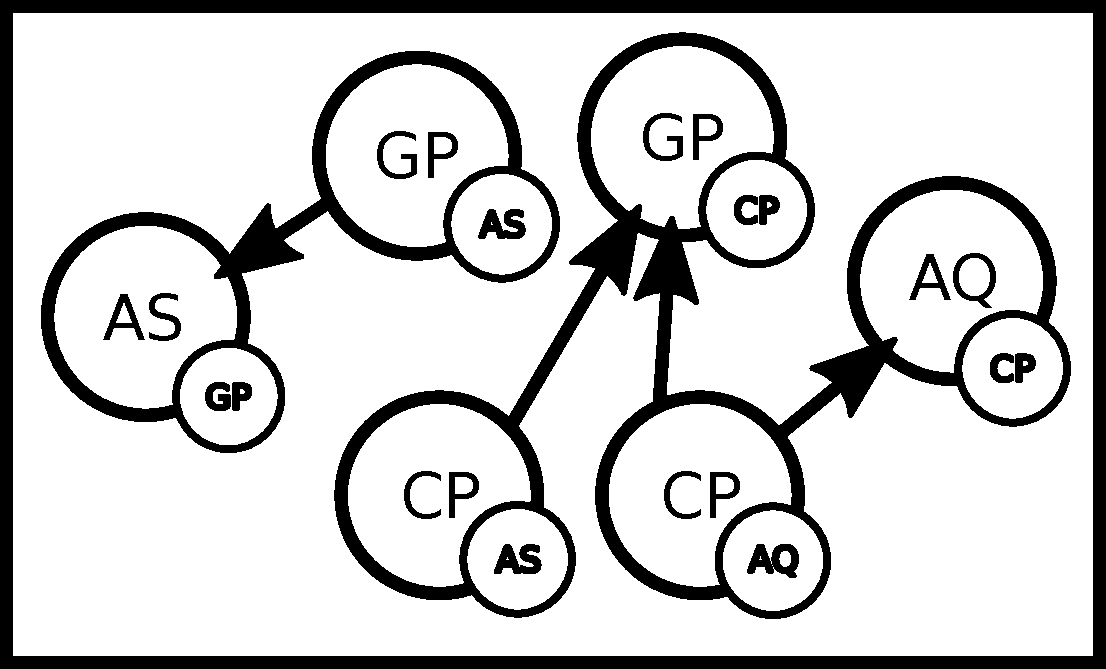
\includegraphics[width=0.3\linewidth]{ex-multilayer-03.pdf}
        \label{fig:ex-multilayer3}
    }
    \caption{Exemplo de uma rede com 4 nós e 4 trigramas (8 conexões). Os nós são GP - \textit{Gerente de Projetos}, AS - \textit{Analista de Sistemas}, AQ - \textit{Arquiteto} e CP - \textit{Coordenador de Projetos}. A mesma rede usando camadas para representar dois níveis de memória é exibida na Figura~\ref{fig:ex-multilayer2}, cada camada representa o nó anterior da conexão e cada imagem do nó na camada é chamado de \textit{nó-estado}. A projeção das camadas de volta para uma rede de camada única está na Figura~\ref{fig:ex-multilayer3}, as anotações em cada nó indicam a camada daquele nó-estado.}
    \label{fig:ex-multilayer-camadas}
\end{figure}

O exemplo da Figura~\ref{fig:ex-multilayer-camadas} mostra a rede formada pelas ocupações \enquote{Arquiteto}, \enquote{Analista de Sistemas}, \enquote{Coordenador de Projetos} e \enquote{Gerente de Projetos} e suas representações em camadas. A partir dessa representação é possível projetar uma rede de uma única camada (uma rede \enquote{comum}), criando-se um \textit{nó-estado} para cada nó em cada camada. Ignorando-se nós-estado que não possuem conexões, essa projeção cria um nó-estado para cada conexão de entrada, como pode ser observado na Figura~\ref{fig:ex-multilayer3}.

Uma vez que a probabilidade estacionária é calculada através das conexões de saída, os nós-estado que possuem saída para os mesmos nós podem ser unificados sem perda de informação para identificação de comunidades. No exemplo da Figura~\ref{fig:ex-multilayer3}, os nós $\text{CP}_\text{AS}$ e $\text{CP}_\text{AQ}$ podem ser unidos em um único nó. \citeonline{Edler2017-kt} chamam essa simplificação de Rede com Memória Esparsa\footnote{no original: \textit{Sparse Memory Network}}.

\begin{figure}[htb]
    \centering
    \subfloat[][Projeção] {
        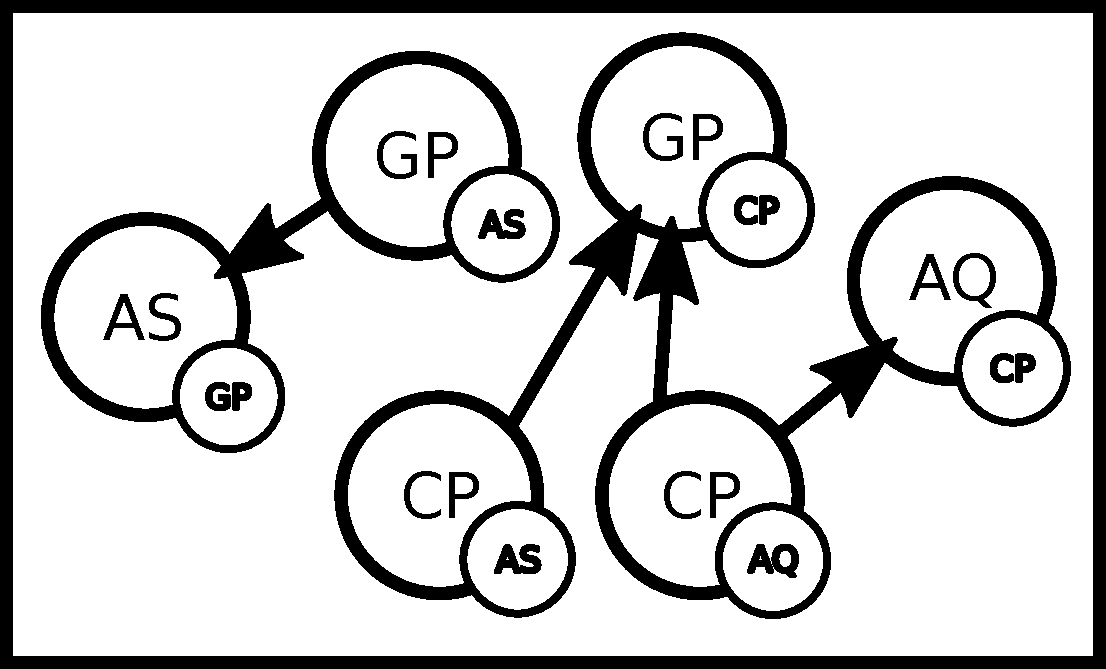
\includegraphics[width=0.3\linewidth]{ex-multilayer-03.pdf}
        \label{fig:ex-multilayer-projecao}
    }
    \subfloat[][Rede com Memória Esparsa] {
        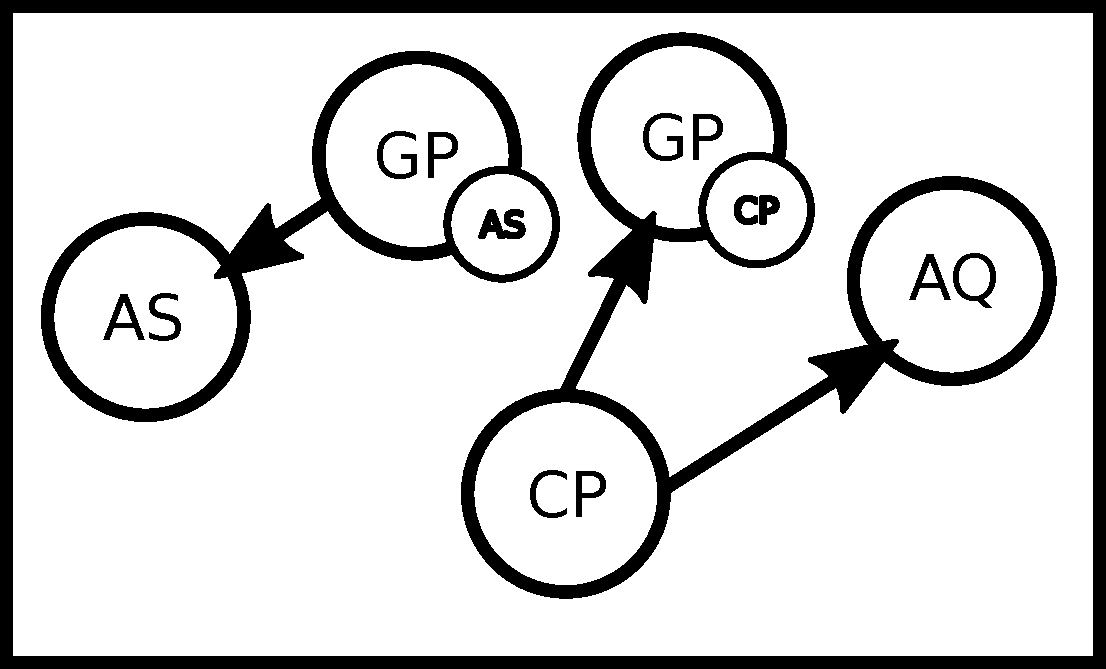
\includegraphics[width=0.3\linewidth]{ex-multilayer-06.pdf}
        \label{fig:ex-multilayer-esparsa}
    }
    \caption{A rede pode ser simplificada unificando nós que possuem saída para os mesmos nós-estados, criando uma Rede com Memória Esparsa~\cite{Edler2017-kt}}
    \label{fig:ex-multilayer-memoria}
\end{figure}

Dessa forma, a aplicação da Equação de Mapa (Equação \ref{eq:map-equation}) permanece a mesma, bastando que os nós-estado que permanecem na mesma comunidade compartilhem o mesmo código. Para isso, a probabilidade estacionária $p_{\alpha_i}$ do nó $\alpha$ na comunidade $i$ passa a ser a soma das probabilidades dos nós-estado $\alpha^s$ de $\alpha$ que estão na mesma comunidade $i$ em qualquer camada $S$,

\begin{equation*} \label{eq:page-rank-multilayer}
\pi_{\alpha_i} = \sum_{s \in S} p_{\alpha_i^s}\,.
\end{equation*}

Substituindo a probabilidade estacionária na Equação~\ref{eq:eta-p}, $H(\mathcal{P}^i)$ passa a ser

\begin{equation*}
H(\mathcal{P}^i) = - \frac{q_{i \curvearrowright}}{p^i_\circlearrowright} \log_2 \frac{q_{i \curvearrowright}}{p^i_\circlearrowright} 
-  \sum_{\alpha \in i} \frac{\pi_{\alpha_i}}{p^i_\circlearrowright} \log_2  \frac{\pi_{\alpha_i}}{p^i_\circlearrowright}\,.
\end{equation*}


(EXPANDIR) Comunidade com sobreposição (ocupações de migração?)

%=============================
\section{CONCEITOS SOBRE CARREIRA}

Segundo~\citeonline{Arthur1989-rn}, carreira é \foreignquote{english}{uma sequência evolutiva da experiência profissional de uma pessoa no tempo}\footnote{No original: \enquote{an evolving sequence of person's work experience over time}.}. Apesar das discussões sobre as mudanças nos modelos de carreira, passando de um modelo linear e centrado na organização para um modelo centrado no indivíduo, as definições de carreira são frequentemente associadas à progressão profissional do indivíduo~\cite{Baruch2004-oy,Sullivan2009-xb,Bendassolli2009-bg}.

Para os fins desse trabalho, define-se carreira como \textit{a sequência de \textbf{ocupações} pela qual um indivíduo passa em sua vida profissional}. Essa definição é similar à de \citeonline{Arthur1989-rn}, porém, limita sua abrangência e a torna mais concreta. Isso permite uma análise menos subjetiva, uma vez que ocupações profissionais podem ser extraídas de currículos e analisadas quantitativamente. No entanto, ela se torna mais limitada, já que essa definição exclui aspectos psicológicos ou sociais.

Essa pesquisa empresta o conceito de \textit{fronteiras de carreira} (\textit{career boundaries}) descrito por \citeonline{Gunz2007-hr} para dar significado ao trabalho. A fronteira de carreira significa que uma mudança entre ocupações nem sempre pode ser realizada livremente. Por exemplo, um profissional precisa de graduação especializada antes de poder se mover da ocupação de \enquote{Auxiliar de Jardinagem} para \enquote{Médico}, por outro lado, a barreira para o mesmo profissional exercer a ocupação de \enquote{Jardineiro} se limita à experiência. É possível perceber que as barreiras não são simétricas, em tempos de crise econômica é mais simples para um \enquote{Engenheiro} tornar-se um \enquote{Corretor de Imóveis} do que o contrário.

As barreiras não se limitam ao conhecimento, quaisquer dificuldades na movimentação podem criar fronteiras. Por exemplo, alguém morando em um grande centro urbano dificilmente exerceria a ocupação de \enquote{Agricultor} sem mover-se para o campo. Um \enquote{Diretor Financeiro} precisaria adequar seu padrão de vida antes de uma transição para uma ocupação com ganhos mais modestos. Uma profissão que está desaparecendo, como \enquote{Contínuo}, possui barreiras mais altas do que uma nascendo, como \enquote{Analista de Experiência do Usuário}.

Um dos pontos principais desse trabalho está na argumentação de \citeonline{Gunz2007-hr} sobre como uma fronteira subjetiva se torna objetiva. Em sua argumentação as fronteiras de carreira são subjetivas e pessoais, onde cada um tem para si quais transições podem ser feitas em sua própria carreira. No entanto, elas se tornam objetivas quando um número suficientemente grande de pessoas possui a mesma compreensão sobre essas transições, a ponto dela ser perceptível em um nível macroscópico. Dessa maneira, as fronteiras de carreira são definidas objetivamente quando uma quantidade suficiente de pessoas entra em \textit{consenso} sobre quais são as transições incomuns.

Partindo desse pressuposto, a identificação de trajetórias comuns e incomuns é condição suficiente e necessária para a detecção de fronteiras entre carreiras. Suficiente, pois a própria definição de fronteira é dependente da identificação do que são transições \enquote{incomuns}. Necessária, pois não existem fronteiras objetivamente definidas sem o consenso.

Essas fronteiras isolam algumas ocupações das outras, criando um grupo coeso pelo distanciamento dos outros grupos e não por alguma característica intrínseca.  Ou seja, a fronteira define o grupo, e não o contrário~\cite{Gunz2007-hr,Abbott1995-ft}. 

No presente trabalho esses aglomerados de ocupações são chamados \textit{ilhas de ocupações} ou \textit{ilhas ocupacionais}, refletindo a facilidade de movimentação dentro de suas fronteiras e o distanciamento de outros grupos.

Como será visto a seguir, as ocupações serão representadas por nós em um grafo, enquanto as conexões trarão informações sobre as transições entre ocupações. Neste tipo de representação, outro conceito central introduzido para o desenvolvimento da pesquisa é o de \textit{polos ocupacionais}, ou seja, ocupações dentro de uma ilha por onde passa o maior fluxo de profissionais. Dada a topologia em formato de estrela encontrada nas ilhas, é esperado que perturbações nesses nós, como aumento ou diminuição no fluxo de profissionais, afetem a rede como um todo e suas eliminações causem o esfacelamento da ilha. Ou seja, os polos ocupacionais são os principais responsáveis por manter a ilha coesa.

%=============================
\section{O MAPA DE CARREIRAS}

\subsection{Introdução}

O Mapa de Carreiras (MCar) traz o resumo da trajetória profissional de cerca de 10 milhões de pessoas e uma de suas manifestações pode ser vista no site \url{http://www.vagas.com.br/mapa-de-carreiras} (Figura~\ref{fig:exemplo-grafo}). Internamente, essas informações estão armazenadas em um grafo e são periodicamente atualizadas. Nesse grafo, os vértices representam \textit{ocupações} e as arestas representam as \textit{movimentações} dos profissionais entre ocupações.

\begin{figure}[ht]
  \centering
  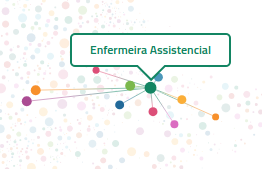
\includegraphics[scale=0.8, frame]{mapa-enfermeira-assistencial.png}
  \caption{Recorte parcial do MCar focando uma ocupação.}
  \source{Mapa de Carreiras}
  \label{fig:exemplo-grafo}
\end{figure}

% TODOS OS EXMPLOS DEVERIAM SER DA ÁREA QUE VAMOS ABORDAR, OU SEJA, TI. ISSO TRAZ MAIS DIDÁTICA E FOCO AO DOCUMENTO.

No contexto do Mapa de Carreiras, uma \textit{ocupação} significa uma atividade profissional, remunerada ou não. A maior parte dessas ocupações são profissões remuneradas, tais como \enquote{Babá} ou \enquote{Arquiteto}. Entretanto, algumas delas aparecem como atividade principal de uma pessoa, mas não são necessariamente uma profissão, tais como \enquote{Mestrando}, \enquote{Enfermeiranda} ou \enquote{Voluntário}. Os vértices possuem diversos atributos que são resumos estatísticos daquela ocupação, tais como a distribuição salarial, a distribuição do tempo de permanência em uma ocupação, entre outras.

% ENTÃO UM VÉRTICE NA VERDADE SERÁ UM VETOR DE CARACTERÍSTICAS COM ESSAS INFORMAÇÕES. PRECISAMOS DEFINIR EXATAMENTE QUAIS CARACTERÍSTICAS COMPORÃO O VETOR DE CARACTERÍSTICAS DOS VÉRTICES. Ronie: Coloco isso dentro da Metodologia?
% COLOQUE A DESCRIÇÃO (VETOR DE CARACTERÍSTICAS) DO VÉRTICE AQUI MESMO.

As arestas que conectam as ocupações representam \textit{movimentações} entre elas, ou seja, o fluxo de pessoas que exercia uma certa ocupação e passou a exercer outra. Acompanhar as arestas permite observar o movimento dos profissionais em suas carreiras. O peso das arestas é o número de profissionais que fizeram a trajetória de uma ocupação para outra. A Figura~\ref{fig:exemplo-medico-do-trabalho} exibe as arestas a partir da ocupação \enquote{Médico do Trabalho}, como exibidas pelo site do Mapa da Carreiras.

\begin{figure}[ht]
  \centering
  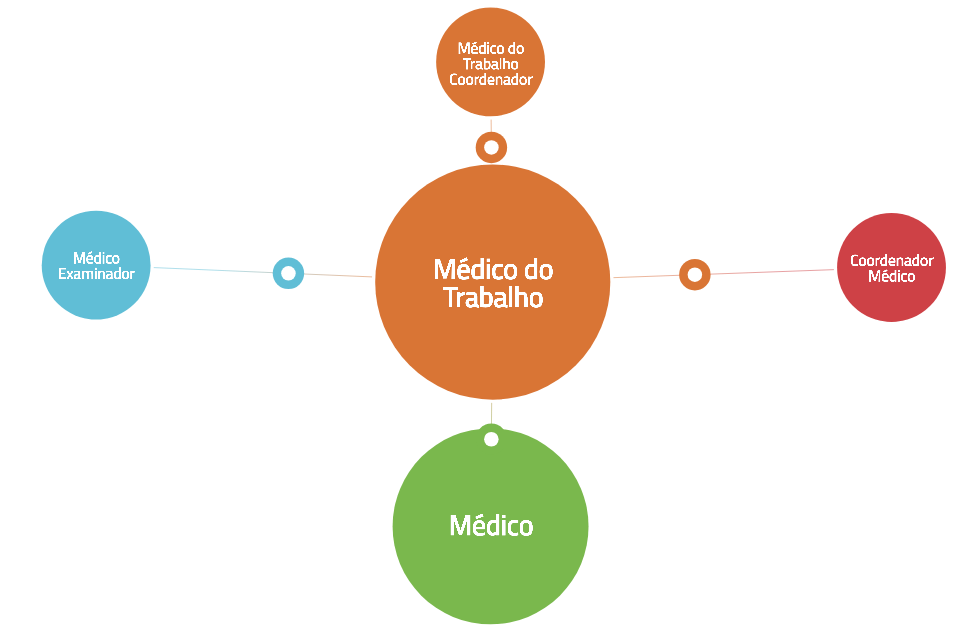
\includegraphics[scale=0.25]{mapa-medico-do-trabalho.png}
  \caption{Ocupações diretamente relacionadas a Médico do Trabalho}
  \source{Mapa de Carreiras}
  \label{fig:exemplo-medico-do-trabalho}
\end{figure}

% TODOS OS EXMPLOS DEVERIAM SER DA ÁREA QUE VAMOS ABORDAR, OU SEJA, TI. ISSO TRAZ MAIS DIDÁTICA E FOCO AO DOCUMENTO.

É importante esclarecer que a visualização observada no site do Mapa da Carreiras foi construída para permitir uma navegação simplificada para o usuário. Para essa pesquisa, os dados utilizados são os mesmos, mas em formatos mais adequados ao projeto. Por exemplo, o equivalente da Figura~\ref{fig:exemplo-medico-do-trabalho} utilizada para análise exploratória pode ser vista na Figura~\ref{fig:grafo-medico-do-trabalho}. Nela, é possível observar ocupações que não estão diretamente relacionadas a \enquote{Médico do Trabalho}, mas que estão no mesmo agrupamento, como \enquote{Médico Plantonista}.

\begin{figure}[ht]
  \centering
  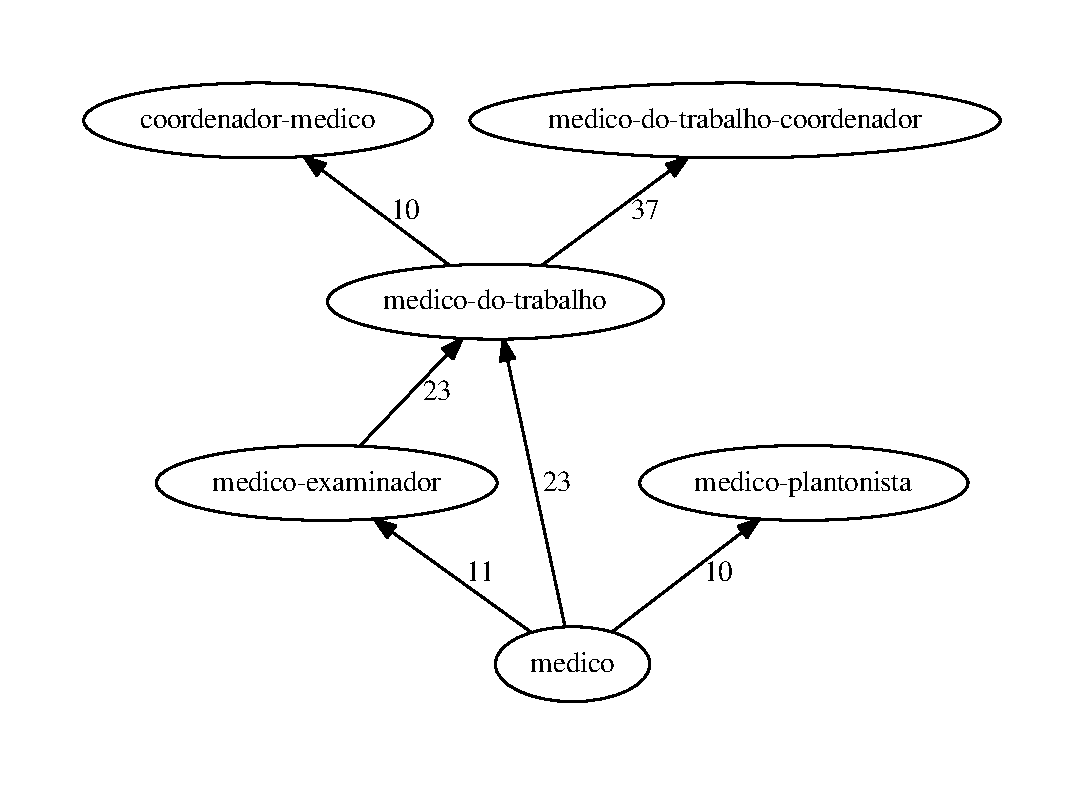
\includegraphics[scale=0.6]{cluster_24.pdf}
  \caption{Subgrafo ao redor de Médico do Trabalho.}
  \source{Elaboração do autor}
  \label{fig:grafo-medico-do-trabalho}
\end{figure}

O grafo do MCar é direcionado e, portanto, o fluxo de profissionais entre ocupações possui uma direção específica, mas é comum que existam movimentações em ambos os sentidos entre duas ocupações. Esse movimento é representado por duas arestas diferentes, mesmo que no site ela seja representada por uma única aresta. Em outras palavras, o MCar é um grafo direcionado, ponderado e com ciclos, porém sem laços.

Por conta dos ciclos, não é possível criar uma ordenação topológica que represente uma clara progressão de carreira para o grafo como um todo. Entretanto, é possível extrair grupos de ocupações que possuem movimentações mais frequentes entre si. Esses agrupamentos são comumente acíclicos, o que possibilita traçar essa progressão entre as ocupações que o compõem. Analisando-se os dados, é possível observar que essa característica é mais frequente em grupos formados por ocupações que requerem maior qualificação técnica, como \enquote{Comércio Exterior} ou \enquote{Médico do Trabalho}, como exibido na Figura~\ref{fig:grafo-medico-do-trabalho}. Já nas ocupações ditas \enquote{operacionais}, o fluxo de movimentação entre ocupações acentua a característica cíclica do grafo. Particularmente, é possível observar um forte ciclo entre as ocupações \enquote{Recepcionista}, \enquote{Vendedor} e \enquote{Auxiliar Administrativo}, como mostrado na Figura~\ref{fig:grafo-ciclo-operacional}.

\begin{figure}[ht]
  \centering
  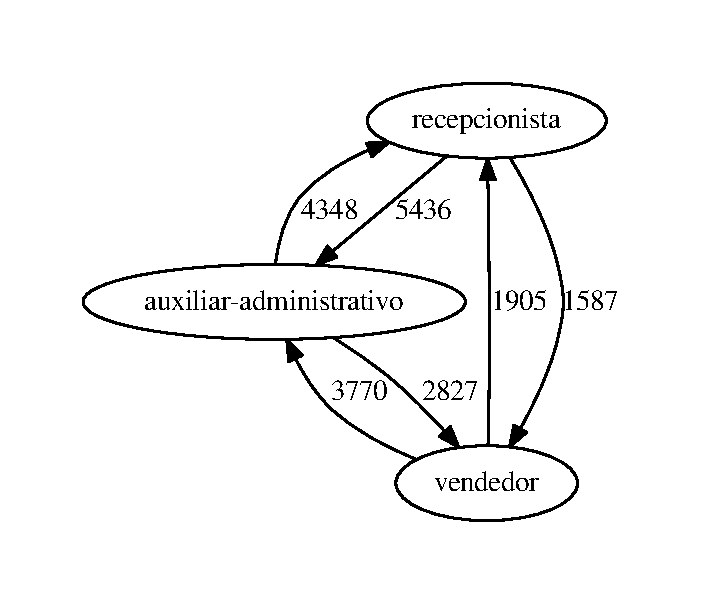
\includegraphics[scale=0.8]{ciclo-operacional.pdf}
  \caption{Ciclo entre Ocupações}
  \source{Elaboração do autor}
  \label{fig:grafo-ciclo-operacional}
\end{figure}

Para a construção dos vértices, os textos presentes nos títulos dos históricos profissionais dos currículos foram \enquote{normalizados}. Nesse contexto, \enquote{normalização} significa transformar os títulos com o mesmo significado na mesma representação textual. Por exemplo, a mesma ocupação pode ter sido registrada por pessoas diferentes como \enquote{Moto Boy}, \enquote{moto boy}, \enquote{Motoboy}, \enquote{Moto Girl} entre outras variações. O que chamamos de \enquote{normalização} é o trabalho de transformar essas diferentes grafias em uma única classe que possa ser usada para identificação da ocupação. No caso, todas as anteriores são normalizadas para \enquote{motoboy}. Esse trabalho também inclui a correção ortográfica e a remoção de abreviação das ocupações.

Após a normalização são criados pares de ocupações cronologicamente ordenados. Isso significa que o término de uma ocupação precisa coincidir com o início da seguinte. Uma margem de dois meses de tolerância na sobreposição corrige pequenas imprecisões na anotação dos históricos profissionais. Currículos com apenas uma ocupação são descartados, bem como ocupações que se sobreponham cronologicamente ou que estejam separadas por um intervalo de tempo maior que um ano.

Os pares de ocupações são unificados produzindo as arestas e os vértices, e as arestas menos relevantes do grafo, ou seja, aquelas com menos de dez movimentações, são podadas. Esse critério de poda foi definido empiricamente através de análise por amostragem. Números muito maiores removem vértices de ocupações mais especializadas como \enquote{Comandante} ou \enquote{Engenheiro de Minas}, enquanto números muito menores acrescentam vértices espúrios causados por erros de grafia que a fase de correção ortográfica foi incapaz de detectar.

Um dos efeitos indesejados desse processo é que algumas ocupações legítimas são removidas do grafo. É o caso de ocupações muito recentes, muito especializadas, ou que ainda não possuem uma concordância da nomenclatura entre os profissionais da área. Como exemplo podemos citar \enquote{Especialista em Experiência do Usuário}, uma profissão recente, que também é chamada \enquote{Analista de UX} ou apenas \enquote{UX}.

% NÃO DEVERÍAMOS CRIAR UM DICIONÁRIO DE EQUIVALÊNCIA DE NOMENCLATURA E SUBTITUIR AS MÚLTIPLAS NOMENCLATURAS POR UMA PADRÃO?
% Ronie: Dá até para fazer manualmente, mas resisto a isso. O motivo pode ser exemplificado pelas ocupações "Analista de Inteligência de Negócios"  e "Analista de BI (Business Intelligence)", apenas o termo traduzido ou um estrangeirismo, entretanto analisando a nuvem de palavras é possível ver que são funções bem diferentes. E olha que é da nossa área e deveríamos saber disso >_<
% Links abaixo:
% http://www.vagas.com.br/mapa-de-carreiras/cargos/analista-de-bi/0
% http://www.vagas.com.br/mapa-de-carreiras/cargos/analista-de-inteligencia-de-negocios/0

Duas outras limitações no grafo ocorrem por conta da experiência profissional ser um campo de texto livre, ou seja, o usuário digita livremente sua ocupação sem estar restrito a uma lista de opções. A primeira se refere a ocupações que foram digitadas para representar uma ocupação dupla, como \enquote{Caixa e Balconista} ou \enquote{Atendente/Estoquista}. A segunda ocorre por ambiguidade no nome da ocupação, como \enquote{Coordenador de Projetos}, que ocorre na carreira de Desenvolvimento de Software e na de Engenharia Civil.

Por outro lado, o campo de texto livre permite a captura de ocupações que pouco provavelmente apareceriam em uma lista curada, como \enquote{IRLA} (Instalador Reparador de Linhas Aéreas) ou \enquote{Rigger} (pessoa no solo que orienta o posicionamento de carga para o operador de guindaste).

Ao final do processo o grafo possui cerca de 8.348 ocupações distintas e 14.031 arestas. Esses números flutuam dependendo das atualizações dos currículos em que são baseados e no crescimento natural do banco de dados. Os dados utilizados nesse trabalho refletem a base atualizada em Fevereiro de 2017.
% COLOQUE O DIA EXATO DE CAPTURA DOS DADOS, OK?

\subsection{O Processo de Construção do Mapa de Carreiras} \label{sec:construcao}

O Mapa de Carreiras é construído a partir dos currículos de um banco relacional condensando seus dados para formar um grafo de movimentação de pessoas entre as ocupações. A construção do MCar é feita em uma estrutura de \textit{pipeline} em que cada componente trabalha os dados e passa o resultado para o componente seguinte, a Figura~\ref{fig:montagem-do-grafo} mostra esquematicamente o processo. Nessa seção, cada um deles é explicado em detalhes.
%% AQUI NA INTRODUÇÃO SUGIRO COLOCAR UM FLUXOGRAMA COM OS BLOCOS DE CONSTRUÇÃO DO MCAR. NA LINHA ABAIXO MENCIONE QUE CADA SEÇÃO VAI DESCREVER UM BLOCO DO PROCESSO.
% Ronie (2017-06-18) A imagem está um pouco mais abaixo, nesse momento me limitei a colocar apenas uma referência para ela :) Acho que depois podemos ajustar o texto.


\subsubsection{Os Dados}

Os dados fonte para essa pesquisa são currículos anonimizados de usuários do site de carreiras VAGAS.com.br. Esses currículos são armazenados em um banco de dados \textit{Microsoft SQL Server}. No total há cerca de 10 milhões de currículos~\todo{Colocar número exato} armazenados entre 1999 e 2017, mas para esse trabalho apenas os currículos atualizados entre Fevereiro de 2012 e Fevereiro de 2017 são utilizados~\todo{Colocar número exato}.

% FALE AGORA DOS CVS DA ÁREA DE TECNOLOGIA. QUANTOS SÃO? QUANTAS E QUAIS SÃO AS CARREIRAS (A LISTAGEM DAS CARREIRAS PODE VIR COMO UM APÊNDICE)
% Ronie: Focamos ainda na área de tecnologia? Acredito que poderíamos focá-la nos exemplos de carreiras maiores (como análise das redes livre de escala e mundo pequeno) que não são boas com carreiras muito pequenas como as que usei acima para exemplificar alguns grafos. Que acha?
% CONTINUO SUGERINDO PELO MENOS COMEÇARMOS COM A ÁREA DE TECNOLOGIA E, SE FOR O CASO, AMPLIAMOS DEPOIS.

Para as análises a serem explicadas nesse capítulo, os dados são primeiramente extraídos para arquivos texto e só então processados. Existem dois formatos usados nesse trabalho. O primeiro formato é descrito por \citeonline{Van_Dongen2008-kx} como \enquote{formato ABC}. Cada linha representa uma aresta, e cada aresta possui três campos separados por um ou mais espaços. Em um grafo direcionado, o primeiro campo é a aresta de partida, o segundo é a aresta de chegada e o campo final representa o peso da aresta. No caso do MCar, o peso representa o número de pessoas que se movimentou de uma ocupação à outra. Esse formato é usado na separação de carreiras através da \textit{clusterização} do grafo usando o \textit{Markov Clustering Algorithm} (MCL)~\cite{Van_Dongen2000-qm} e na montagem de visualizações exploratórias usando o programa \enquote{Graphviz}~\cite{Gansner2000-oo}.

\vspace{\abovedisplayskip}

\noindent
\begin{minipage}{\linewidth}
\begin{lstlisting}[frame=single,caption=Arquivo em Formato ABC,label=lst:formato-abc,captionpos=b]
medico-examinador medico-do-trabalho 23
medico-do-trabalho coordenador-medico 10
medico-do-trabalho medico-do-trabalho-coordenador 37
medico medico-plantonista 10
medico medico-examinador 11
medico medico-do-trabalho 23
\end{lstlisting}
\end{minipage}

O segundo formato é uma lista de registros onde cada um ocupa uma única linha. Cada registro é codificado como um \textit{array} de atributos no formato JSON (\textit{Javascript Object Notation}). Esse formato é usado em várias etapas da montagem do MCar e seu conteúdo varia de etapa para etapa. Os campos relevantes são descritos nas respectivas seções a seguir.

\subsubsection{O Processamento da Informação}

O volume de dados e a variedade de análises desse trabalho impõe algumas restrições de ordem prática. O volume de dados é grande o suficiente para exceder a memória de um computador convencional, algumas das ferramentas utilizadas não se comunicam com outras exceto através de arquivos texto e o tempo para processamento facilmente excede alguns dias se os processadores não forem adequadamente utilizados.

Essas restrições e a necessidade de atualizar continuamente os dados do MCar levaram a implementação de um sistema que executasse todos os passos para sua montagem de maneira automática.

A informação é processada em uma série de etapas consecutivas usando um padrão arquitetural conhecido como \textit{Dataflow}~\cite{Carkci2014-jk, Hohpe2003-nj}, especificamente o modelo conhecido como \textit{Pipes and Filters} ou \textit{Pipeline}. Nesse padrão, os dados fluem continuamente de um processo para o outro, sendo transformados e filtrados conforme o processo avança. 

Em uma estrutura de \textit{pipeline}, com exceção de alguns componentes especiais, cada processo possui apenas uma interface de entrada e uma interface de saída. Desde que mantenha a mesma interface, um processo pode ser substituído por outro, ou por um conjunto deles, sem afetar outras partes do sistema.

Essa arquitetura foi implementada em máquinas \textit{Linux} utilizando \textit{pipes} e \textit{sockets} para comunicação interprocessos. Um \textit{pipe} no \textit{Linux} é uma implementação de FIFO em memória RAM. A interface para \textit{push} na fila é idêntica a gravação de uma linha de texto em um arquivo. Do outro lado um outro processo lê a fila com a mesma interface de leitura de um arquivo linha a linha. Por usar interfaces compatíveis que leituras e gravações em arquivo, qualquer programa capaz de executar essas operações pode ser usado como parte do \textit{pipeline}. Isso resolve o problema do uso de ferramentas díspares, desde que sejam capazes de gravar e ler em arquivos texto, são capazes de se integrar ao processo como um todo.

Enquanto \textit{pipes} permitem a comunicação interprocessos na mesma máquina, \textit{sockets} podem ser usados para comunicação entre computadores através de uma interface padronizada. Ao invés dos \textit{sockets} nativos do \textit{Linux}, optou-se pelo \textit{ZeroMQ} que é uma implementação mais robusta, criada para transmitir dados usando diversos modelos de distribuição~\cite{Hintjens2013-tz}.

O \textit{ZeroMQ} possui interfaces para diversas linguagens de programação, mas para preservar a interface entre processos foram criados componentes que traduzem a entrada em \textit{pipes} para \textit{sockets ZeroMQ} e vice-versa. Em termos práticos, a comunicação entre processos pode ser feita entre processos da mesma máquina ou entre diferentes computadores de maneira transparente.

A maior parte dos processos foi implementada usando a linguagem Ruby, mas alguns processos foram implementados usando Python ou programas específicos, como o MCL para \textit{clusterização} e o Graphviz para posicionamento do grafo em um plano bidimensional.

O processo de montagem do grafo está resumido no fluxo apresentado na Figura~\ref{fig:montagem-do-grafo}.

\begin{figure}[ht]
  \centering
  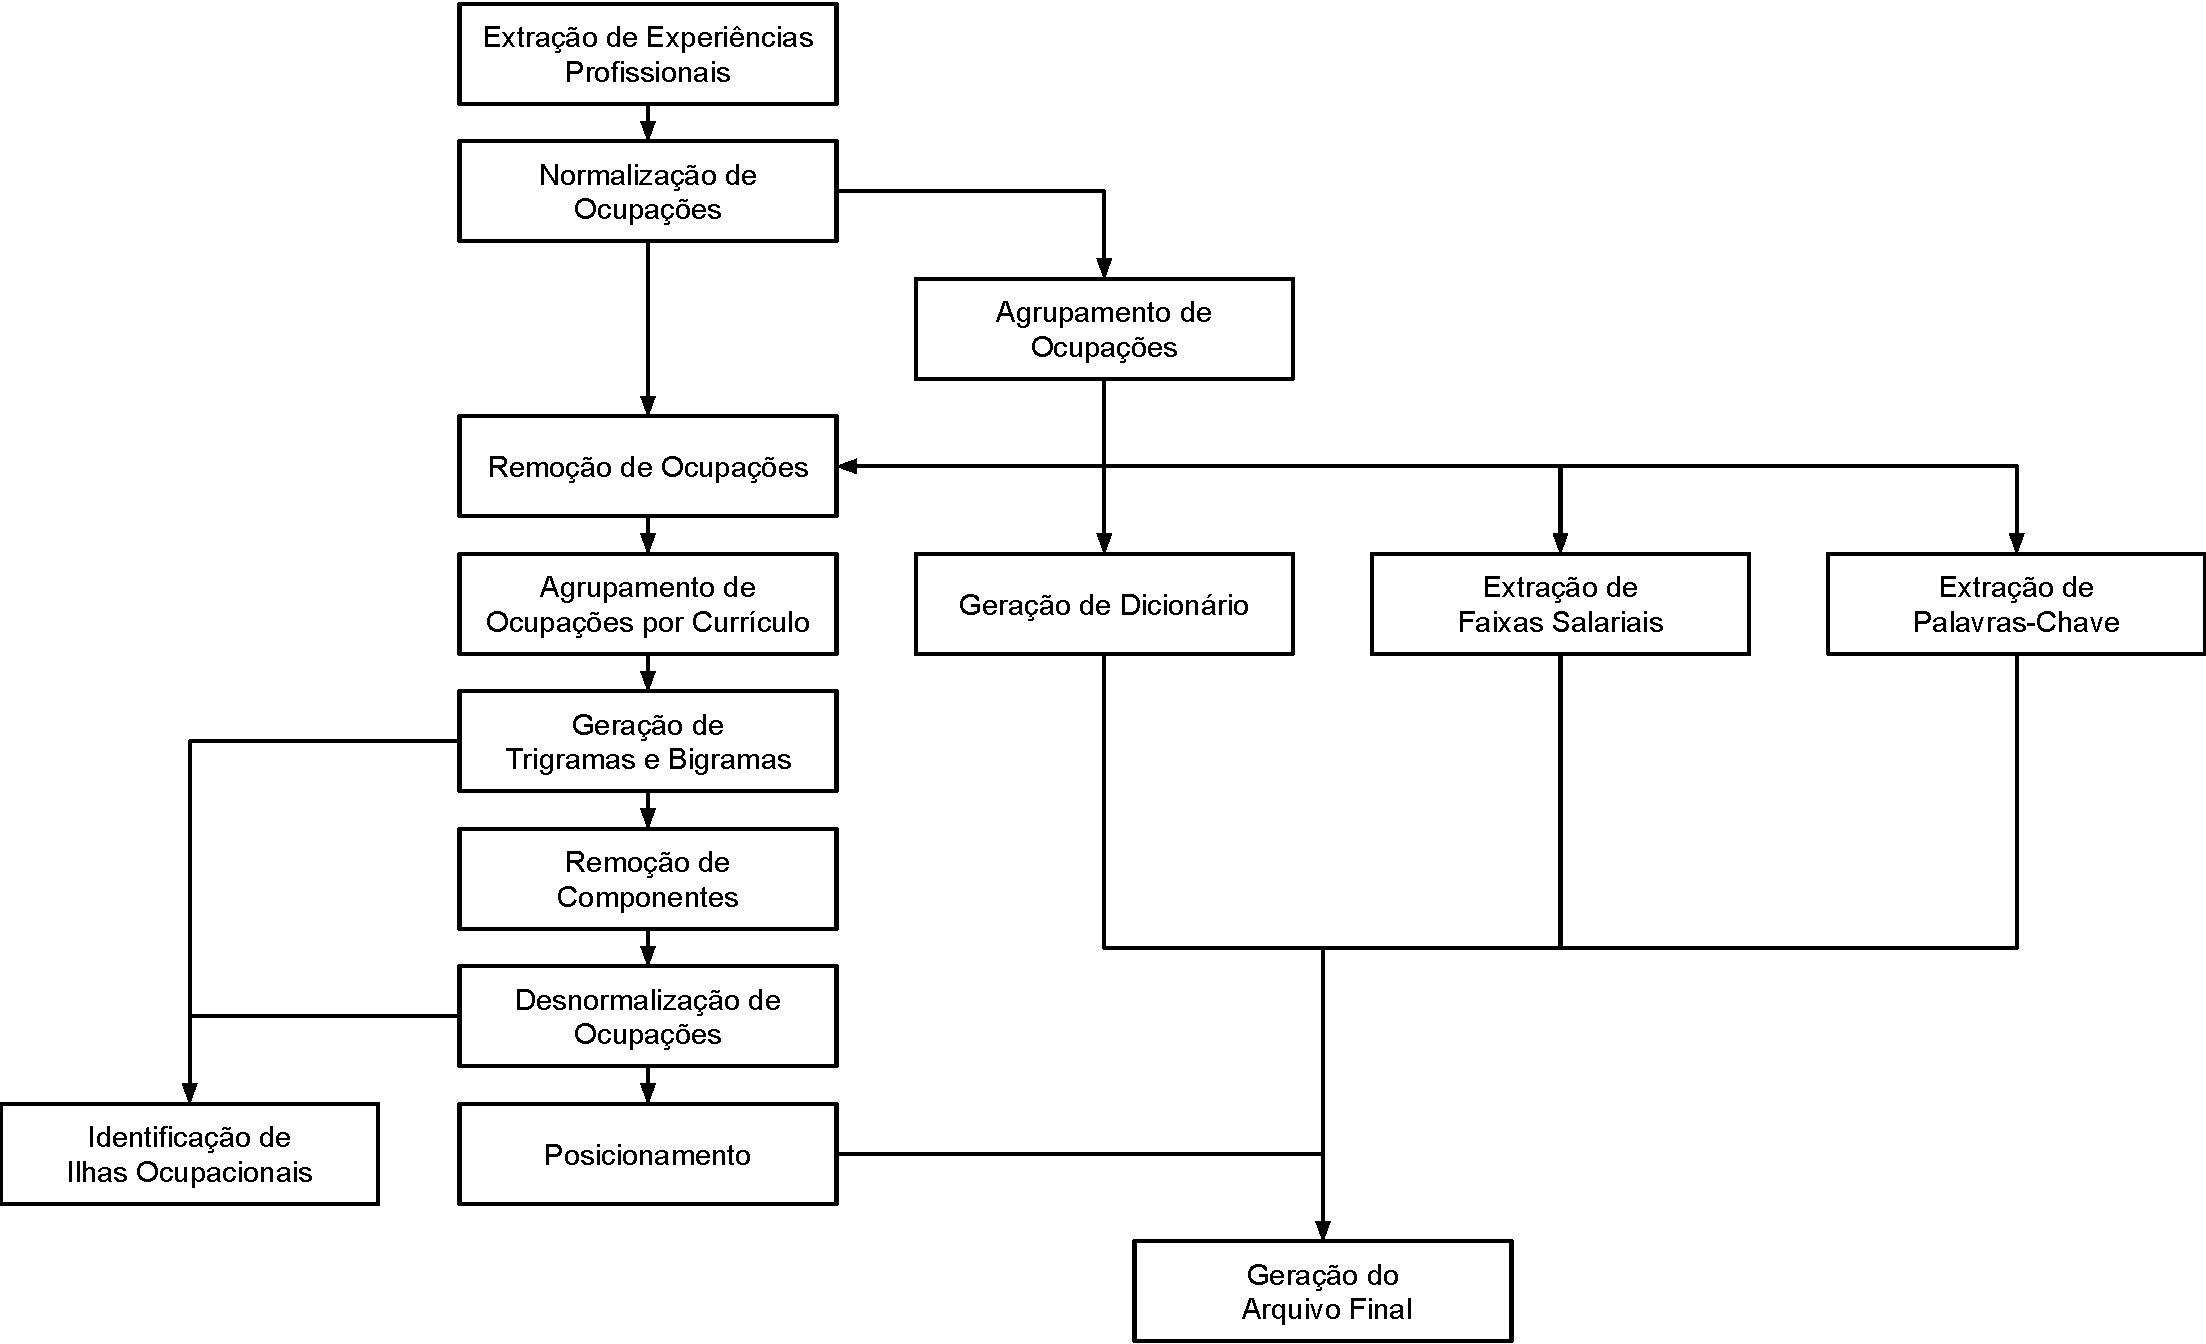
\includegraphics[scale=0.4]{pipeline1.pdf}
  \caption{Montagem do Grafo}
  \label{fig:montagem-do-grafo}
\end{figure}

\subsubsection{Extração das Experiências Profissionais} \label{sec:extracao-experiencia}

O primeiro processo do \textit{pipeline} extrai os registros do banco de dados relacional e os grava em arquivos texto. O processo não extrai currículos, mas sim experiências profissionais. Cada registro representa uma única experiência.

Os dados extraídos são:

\begin{description}

  \item[Identificador do Currículo] é um número único para cada currículo dentro do banco de dados. Ele é usado posteriormente para agrupar as experiências profissionais por pessoa.

  \item[Nome da Ocupação] é o texto digitado livremente pelo usuário no campo nomeado \enquote{Cargo} no currículo. Esse texto dá origem aos nomes das ocupações usadas no Mapa de Carreiras.

  \item[Data de Início] e \textbf{Data de Término} marcam quando o profissional iniciou naquela ocupação e até quando a exerceu. Se é a ocupação atual, não existe uma data de término. Esses campos são usados para determinar a sequência de experiências profissionais que formarão as arestas do grafo.

  \item[Texto Descritivo] é o texto digitado livremente pelo usuário no campo com o nome \enquote{Descrição} no currículo. Esse campo é usado para criar uma nuvem de palavras-chave sobre a ocupação.

\end{description}

\subsubsection{Normalização de Ocupações} \label{sec:normalizacao}

Nessa etapa, o nome da ocupação é normalizado para uma classe de maneira que todas as grafias significando a mesma ocupação sejam transformadas em uma mesma classe. Nessa pesquisa a classe é chamada \enquote{classe equivalente} ou \enquote{ocupação normalizada}.

Para transformar o texto digitado em uma ocupação normalizada os erros de digitação são corrigidos, pontuações são removidas, abreviaturas frequentes são expandidas, o texto é colocado em minúsculas, é feita a singularização das palavras que compõem a ocupação e os nomes são masculinizados (\enquote{secretária} se transforma em \enquote{secretário}, por exemplo).

Ocupações com múltiplas palavras também são ordenadas alfabeticamente. Dessa forma, ocupações como \enquote{Auxiliar Financeiro-Administrativo} e \enquote{Auxiliar Administrativo-Financeiro} resultam na classe \enquote{administrativo auxiliar financeiro}.

As classes resultantes lembram vagamente o termo original, como no exemplo acima. No processo descrito na Seção~\ref{sec:criar-dicionario}, é criado um dicionário entre a classe equivalente e um nome que tenha significado para o usuário.

\subsubsection{Remoção de Ocupações Incorretas} \label{sec:remocao-ocupacoes-incorretas}

Mesmo após a remoção de casos únicos, alguns nomes presentes nesse campo podem não ser considerados ocupações. São erros comuns que a etapa de normalização não é capaz de corrigir ou representam um entendimento equivocado por parte do usuário.

Casos emblemáticos são os textos \enquote{sim}, \enquote{não} ou \enquote{o mesmo} encontrados no campo destinado ao nome da ocupação. A remoção desses casos precisou ser feita manualmente, ou seja, especialistas da empresa revisaram a lista de ocupações e criaram um dicionário com os erros mais comuns utilizados nessa etapa do processo. Esse dicionário foi aprimorado com sugestões dos usuários após a publicação do MCar.

\subsubsection{Agrupamento de Ocupações por Currículo}

As ocupações são agrupadas por currículo, formando uma sequência cronológica das experiências de um profissional. Até essa etapa, há uma experiência profissional por registro, após ela, cada registro contém uma sequência de experiências profissionais do mesmo indivíduo, ordenadas cronologicamente.

% Inserir um diagrama com os campos. Ronie 2017-04-30

\subsubsection{Remoção de Experiências sem Conexão ou Sobrepostas}

Como o objetivo final é criar um grafo que sumarize o \textit{movimento} de pessoas entre ocupações, as experiências profissionais que não se conectam cronologicamente com nenhuma outra são removidas. São consideradas desconexas quaisquer experiências em sequência cujo início da posterior esteja a mais do dois meses de distância do fim da anterior.

% Inserir um gráfico explicativo. Ronie 2017-02-30

Na mesma etapa, removem-se experiências profissionais que se sobreponham. Uma vez sobrepostas, não é possível afirmar que uma é sequência natural da outra ou que sequer tenham relação entre si. É comum encontrar no banco de dados carreiras paralelas em que gestores também são professores ou técnicos que também sejam voluntários. Da mesma maneira que experiências desconexas, as que se sobrepõem por mais de dois meses são removidas.

\subsubsection{Remoção de Currículos sem Experiência}

Após o processo anterior, são removidos os registros que possuam apenas uma ou nenhuma experiência profissional.

\subsubsection{Geração de Pares de Experiências}

As experiências profissionais de cada currículo são pareadas por ordem cronológica. Por exemplo, um currículo que tenha a seguinte sequência de ocupações \enquote{Faxineiro \textrightarrow~Copeiro \textrightarrow~Chapeiro}, produz os pares \enquote{Faxineiro \textrightarrow~Copeiro} e \enquote{Copeiro \textrightarrow~Chapeiro}.

Antes desse processo, cada registro é uma sequência de experiências profissionais. O processo expande cada registro em múltiplos registros, cada um representando um par de experiências profissionais de um único indivíduo.

\subsubsection{Agrupamento de Pares de Ocupações}

Pares iguais de ocupações são agrupados e contados, gerando um \textit{multiset}, ou seja, um conjunto com o número de repetições de cada elemento. O número de repetições em um par representa o número de pessoas que se movimentaram de uma ocupação para outra.

As etapas posteriores podam o grafo em suas arestas menos relevantes e transformam sua representação textual para que possa ser lido por outros programas.

\subsubsection{Remoção de Pares Pouco Frequentes} \label{sec:grafo-final}

A maioria dos pares de ocupações ocorrem pouquíssimas vezes. \todo{Em um conjunto com XX pares, cerca de XX ocorrem apenas uma vez.} Esse pequeno número de repetições é causado tanto por trajetórias incomuns, quanto por erros de digitação que as etapas anteriores não foram capazes de eliminar. Por vezes são apenas ocupações similares a outras, mas onde os usuários escrevem de maneira pouco convencional. Com alguma frequência, os pares realmente representam trajetórias em carreiras extremamente específicas.

Para encontrar um número de corte foi feita uma avaliação manual por amostragem. Amostras com algumas centenas de pares com números de corte entre 1 e 30 foram analisadas por especialistas da empresa junto com o pesquisador. O objetivo foi encontrar um número que não fosse conservador demais, removendo trajetórias válidas, nem liberal demais, permitindo trajetórias com erro.

Após o processo de análise, chegou-se a um número próximo a 10 repetições. Pares de ocupações com menos de 10 repetições são removidos.

A partir desse ponto, os dados para a montagem do grafo estão prontos em formato texto.

\subsubsection{Posicionamento dos Vértices do Grafo}

Para que o grafo possa ser exibido bidimensionalmente, é preciso que seus vértices sejam posicionados de modo a evitar a sobreposição e que os vértices relacionados por arestas de maior peso estejam mais próximos.

O algoritmo de \textit{Force-Directed} é usado para posicioná-los corretamente. Esse algoritmo é aplicado nesse passo utilizando o programa Graphviz. A saída do Graphviz é um arquivo texto com a posição X e Y do vértice em um plano cartesiano.

\subsubsection{Identificação de Carreiras}

%% O QUE É UMA PROTO-CARREIRA?

% Me parece que "proto-carreiras" não é um nome lá muito bom, mas foi o que consegui por enquanto =/ Ronie 2017-04-29
% Aqui também tem uma dose não saudável de especulação baseado no tempo que fiquei olhando para esse grafo. Pode ser o caso de colocar números em tudo (gosto disso), ou eliminar boa parte do texto. Ronie 2017-04-30

O grafo gerado no Passo~\ref{sec:grafo-final} é usado nesse processo para gerar agrupamentos. Entre duas ocupações o maior fluxo de movimentações indica uma certa preferência por uma das duas. Por exemplo, se o número de movimentações entre \enquote{Analista de Sistemas \textrightarrow~Coordenador de Projeto} for maior que o reverso \enquote{Coordenador de Projeto \textrightarrow~Analista da Sistemas}, considera-se que \enquote{Coordenador de Projeto} é uma ocupação que sucede \enquote{Analista de Sistemas}. Algumas vezes o fluxo entre as ocupações é tão similar que não é possível dizer que há uma ordem de sucessão, como no caso apresentado no ciclo de ocupações operacionais na Figura~\ref{fig:grafo-ciclo-operacional}; em outros, o sentido contrário possui um fluxo várias vezes menor ou não há fluxo contrário, como o caso do grafo sobre \enquote{Médico do Trabalho} na Figura~\ref{fig:grafo-medico-do-trabalho}.

\todo[inline]{Ronie: estou pensando que a seção abaixo pode ser movida para \enquote{conclusões} ou mais para frente, que acha?}

Quando o fluxo de pessoas de uma ocupação para outra é relevante, é possível notar que essa ordem de preferência vai normalmente de ocupações mais operacionais e com salários mais baixos para ocupações mais gerenciais e com salários mais altos. Isso coincide com a senso comum de progressão de carreira.

A grosso modo, o agrupamento e o fluxo de migração das ocupações revela o que se pode considerar um \enquote{protótipo de carreira}. Ou seja, um esboço onde um indivíduo em uma ocupação dentro desse grupo tem uma probabilidade maior de se manter nele e de se movimentar para ocupações no topo do grupo.

Existe, no entanto, um grupo que não obedece às características descritas acima. Ao se tentar ordená-lo topologicamente, não há uma ordem de preferência clara entre as ocupações, o que indica que não há uma noção de sucessão como em outros grupos, como exemplificado anteriormente na Figura~\ref{fig:grafo-ciclo-operacional}. Ele também possui algumas ocupações que conectam uma grande quantidade de outras ocupações, como \enquote{Auxiliar Administrativo}.\todo{, que possui movimentações com XX ocupações, cerca de XX\% das ocupações do MCar.}

Ao analisar o grupo, nota-se que a escolaridade mais frequente nessas ocupações é a de \enquote{segundo grau completo}, significando que essas ocupações não necessitam de treinamento especializado para serem desempenhadas, o que é um indício que esse grupo reflete a própria definição de \enquote{operacional}.

Algumas outras ocupações também possuem \enquote{segundo grau completo} como escolaridade mais frequente, mas se comportam como os grupos com uma direção clara de preferência entre as ocupações. Uma análise manual da descrição das suas ocupações e das palavras-chave relacionadas sugere que essas são ocupações \enquote{técnicas}. Ou seja, uma ocupação que requer um treinamento não-trivial, mas não tão exigente quanto uma graduação. Como exemplo, é possível observar a carreira de cozinheiro na Figura~\ref{fig:exemplo-grafo-cozinheiro}.

\begin{figure}[htb]
  \centering
  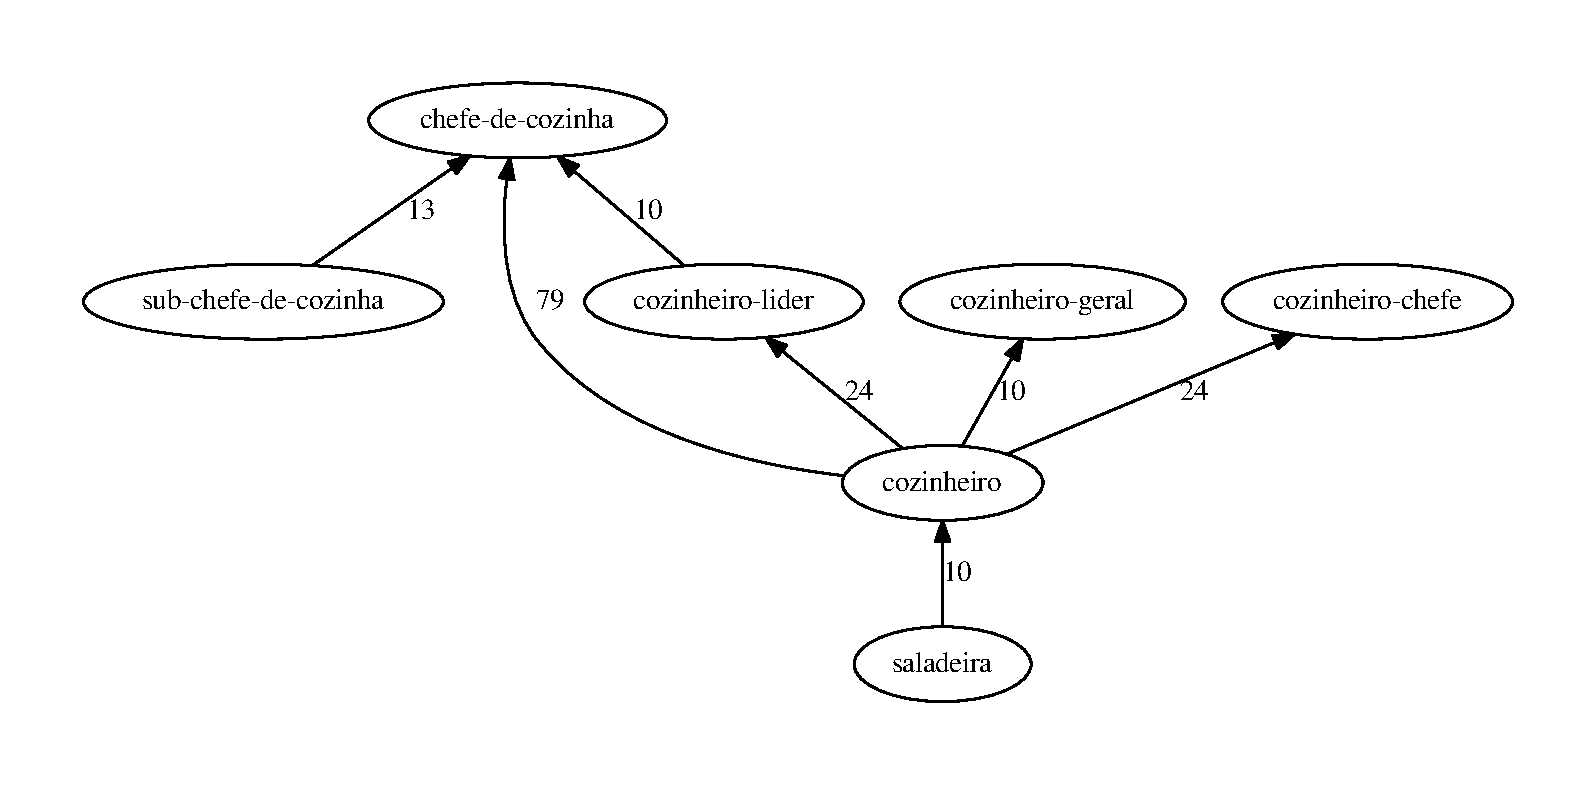
\includegraphics[scale=0.6]{subcluster_01_11.pdf}
  \caption{Carreira Técnica de Cozinheiro}
  \label{fig:exemplo-grafo-cozinheiro}
\end{figure}

%% O QUE DEFINE SEGUIR O CAMINHO "AGRUPAMENTO DE OCUPAÇÕES POR CURRÍCULO" OU "AGRUPAMENTO DE OCUPAÇÕES"?

\subsubsection{Agrupamento de Ocupações}

Esse processo agrupa os dados gerados pelo processo descrito na Seção \ref{sec:remocao-ocupacoes-incorretas} por ocupação. Cada ocupação normalizada agora possui uma lista com suas grafias originais, uma lista com as descrições daquela experiência profissional escrita por cada indivíduo, bem como a quantidade de ocupações agrupadas.

\subsubsection{Remoção de Ocupações com Pouca Frequência}

Mesmo com o processo de correção e normalização, algumas experiências profissionais são escritas de maneira única. Isso pode significar um erro, uma ocupação singular ou o uso de termos pouco convencionais. Como o objetivo da montagem do grafo é extrair as carreiras mais frequentes, os casos únicos podem ser seguramente removidos sem a necessidade de determinar sua causa.

\subsubsection{Criação de Dicionário para Exibição} \label{sec:criar-dicionario}

Os textos resultantes do processo de normalização descrito na Seção~\ref{sec:normalizacao} não são adequados para exibição. Esse processo contabiliza o número de grafias exatamente idênticas para cada ocupação normalizada e assume como \enquote{nome de exibição} a grafia mais frequente.

A limitação desse processo é que algumas ocupações são descritas no masculino ou no feminino dependendo do número de profissionais do gênero exercendo essa ocupação. Por exemplo, uma das ocupações de Direito é descrita como \enquote{Advogado} (no masculino) pois existem um pouco mais profissionais do gênero masculino exercendo a profissão, por outro lado, outra ocupação correlacionada é descrita como \enquote{Advogada Coordenadora} pelo motivo contrário.

Apesar da regra da língua portuguesa do uso do masculino quando há um grupo de gênero misto\todo{ref}, optou-se por não se modificar o gênero artificialmente, preservando a grafia da predominância do gênero na ocupação.

\subsubsection{Extração de Palavras-Chave}

As palavras-chave são extraídas a partir das descrições digitadas pelos usuários no campo \enquote{Experiência Profissional} dos currículos. O processo descrito abaixo tenta criar expressões significativas, ou seja, pequenas frases, que ajudem a descrever o cargo ao invés de apenas indicar as palavras mais comuns. Um fato notável é que não é possível utilizar \textit{stemming} ou correção ortográfica nesse processo, pois existe uma grande quantidade de jargões e siglas específicos nas descrições.

Para formar expressões, são gerados unigramas, bigramas e trigramas para as descrições de cada experiência profissional. A seguir, elas são ordenadas por TF-IDF e as palavras que aparecem repetidas em um n-grama de menor TF-IDF são removidas. Por exemplo, se a palavra \enquote{fiscal} aparece com maior TF-IDF que o bigrama \enquote{nota fiscal}, a palavra \enquote{fiscal} é removida da lista.

% Ronie: na prática, o resultado é muito bom, mas o algoritmo foi baseado no meu nariz =/ Então, talvez eu devesse refazer o processo com uma técnica de sumarização melhor.
\begin{comment}
\subsubsection{Gravação do Arquivo Final}

A definir\ldots
\end{comment}

\subsection{Atributos das Ocupações}

Complementar à montagem do grafo, os vértices com as ocupações são abastecidos com outras informações. São elas:

\begin{description}
  \item[Idade] computada para cada ocupação considerando a data de nascimento do profissional e a data de entrada na ocupação.
  \item[Salário] da ocupação atual corrigido pelo IPCA a partir da última data de atualização do currículo.
  \item[Tempo de Permanência na Ocupação] extraída a partir do número de meses consecutivos do indivíduo naquela experiência profissional.
  \item[Escolaridade] registrada no currículo com as opções 1º, 2º e 3º graus completos.
  \item[Curso de Graduação] registrada a partir de uma lista de cursos, essa informação é coletada apenas para escolaridade acima de 2º grau completo. A graduação é considerada apenas para as ocupações que ocorrem depois do término do curso.
  \item[Gênero] do profissional, apenas masculino ou feminino.
  \item[Número de Profissionais na Ocupação] é obtido contando as ocupações que não possuem data de término.
\end{description}

A idade, o salário e o tempo de permanência são sumarizados usando o \textit{resumo de cinco números}, com seus intervalos de confiança 95\% e uma \textit{estimativa de densidade de probabilidade}. Já a escolaridade, o curso de graduação e o gênero são simples contagens de frequência.

O \textit{resumo de cinco números} consiste no valor mínimo, 1º quartil, mediana, 3º quartil e valor máximo. Esse resumo é proposto por \citeonline{Hoaglin1983-aq} como estatística descritiva de uma amostra.

O intervalo de confiança 95\% para todos os valores do resumo de cinco números é obtido por \textit{bootstrap} com 10.000 iterações. A técnica permite identificar os valores mais confiáveis independentemente do tamanho da amostra e das distribuições.

A Tabela~\ref{tab:resumo-salario-programador} mostra os quartis e seus intervalos de confiança para a ocupação de \enquote{Programador}.

\begin{table}[htb]
    \centering
    \begin{tabular}{r|c|c|c}
        & \textbf{2,5\%} & \textbf{Estimativa} & \textbf{97,5\%} \\ \hline
        \textbf{1º Quartil} & 1672           & 1709                & 1751 \\ \hline
        \textbf{Mediana}    & 2354           & 2403                & 2476 \\ \hline
        \textbf{3º Quartil} & 3225           & 3294                & 3354 \\
    \end{tabular}
    \caption{Quartis para o salário de \enquote{Programador}}
    \label{tab:resumo-salario-programador}
\end{table}

\begin{comment}
A Tabela~\ref{tab:resumo-salario-programador} mostra o resumo e seus intervalos de confiança para a ocupação de \enquote{Programador}.

\begin{table}[htb]
\centering
\begin{tabular}{r|c|c|c}
                    & \textbf{2,5\%} & \textbf{Estimativa} & \textbf{97,5\%} \\ \hline
\textbf{Mínimo}     & [coletar]      & [coletar]           & [coletar] \\ \hline
\textbf{1º Quartil} & 1672           & 1709                & 1751 \\ \hline
\textbf{Mediana}    & 2354           & 2403                & 2476 \\ \hline
\textbf{3º Quartil} & 3225           & 3294                & 3354 \\ \hline
\textbf{Máximo}     & [coletar]      & [coletar]           & [coletar]    
\end{tabular}
\caption{Resumo de 5 números para salário de \enquote{Programador}}
\label{tab:resumo-salario-programador}
\end{table}
\end{comment}

A \textit{estimativa de densidade de probabilidade} é obtida por um Estimador de Densidade de Kernel usando um distribuição gaussiana como função kernel. A largura de banda escolhida para cada estimativa é o menor valor limite para que a distribuição se mantenha unimodal.

\section{UM ESTUDO ANALÍTICO DO MCar USANDO CIÊNCIA DE REDES: RESULTADOS PRELIMINARES} \label{sec:resultados-preliminares}

A comparação de uma rede real com modelos nulos indica fenômenos que não acontecem por aleatoriedade. Essa aplicação é uma análise exploratória que levanta a questão de por que eles acontecem se o acaso não é uma explicação aceitável.

Ao se correlacionar as medidas usadas em Ciência de Redes cria-se mais um conjunto de questões sobre o significado da correlação. Algumas dessas correlações se destacam, pois ecoam com fenômenos conhecidos da movimentação de profissionais, fornecendo hipóteses plausíveis de seu funcionamento.

%% O QUE VOCÊ QUER DIZER COM "AO SE CORRELACIONAR...CRIA-SE MAIS UM CJTO DE QUESTÕES SOBRE O SIGNIFICADO DA CORRELAÇÃO"?

Um estudo confirmatório não é possível apenas com os dados apresentados aqui, pois eles requerem um aprofundamento em ciências sociais que foge da proposta dessa pesquisa. Entretanto, a análise estatística de um grande volume de dados fornece indícios que podem servir como motivadores para pesquisas mais ambiciosas ou podem ser usados como complemento em estudos sociais. Ainda assim, os achados nesse capítulo são plausíveis por construção já que são propostos baseados em medições sobre dados reais.

%% ESSE PARÁGRAFO ACIMA FICOU UM POUCO "ROLANDO LERO"
%% Ronie (2017-08-13) Acho que foi só diminuir o número de adjetivos :D Veja se ficou melhor :)

%% POR QUE NÃO TEMOS DADOS SUFICIENTES PARA VALIDAR, PELO MENOS NO CONTEXTO EM ESTUDO, AS HIPÓTESES COLOCADAS ACIMA.
%% ALÉM DISSO, SE SÃO HIPÓTESES EU SUGIRO QUE AS DESTAQUEMOS COMO TAL E NA PARTE EXPERIMENTAL A GENTE VÁ TENTANDO VALIDÁ-LAS. FIZ O EXERCÍCIO DE CRIAR AS HIPÓTESES ACIMA, VEJA O QUE ACHA. COMO ESSAS HIPÓTESES SE REFEREM AO MCAR, SUGIRO COLOCÁ-LAS EM UMA SEÇÃO SEPARADA E DEIXARMOS AQUI COMO UMA REVISÃO CONCEITUAL. ISSO AJUDA A COMPOR A PROPOSTA DE SUA DISSERTAÇÃO. MUITO INTERESSANTE!!! NA REALIDADE, SUA DISSERTAÇÃO É UMA ANÁLISE EXPLORATÓRIA SOBRE O MCAR E, PORTANTO, A MOVIMENTAÇÃO DE CARREIRA. NESSE SENTIDO, TODOS OS INSIGHTS DEVEM SER DESTACADOS COMO CONTRIBUIÇÃO AO INVÉS DE APARECEREM DILUÍDOS NUM CAPÍTULO DE REVISAO CONCEITUAL
% Ronie: Gostei MUITO! Acho que ficou muito mais claro e a separação faz bastante sentido. Fazemos um capítulo para isso ou colocamos junto com o desenvolvimento, tentando validá-la? 


As hipótese propostas são pontos de partida para diversas aplicações. Por exemplo, a criação de uma classificação de ocupações baseada em agrupamento. É esperado que ela retrate com mais precisão um conjunto de funções em que seus membros compartilham habilidades. Também é possível inferir capacitações através do histórico profissional e compreender com mais clareza a movimentação profissional.

Abaixo, as propostas são enumeradas e justificadas.

\begin{hypothesis}[Atração Profissional]
    A força de entrada do nó (Seção~\ref{sec:forca}) indica o quanto uma ocupação atrai profissionais. Nós de grande força de entrada funcionam como polos atratores de mão de obra, seja pela demanda, seja pela facilidade em exercer a ocupação ou seja por sua atratividade.
\end{hypothesis}

Algumas ocupações, como \enquote{Auxiliar Administrativo}, possuem um grande número de profissionais em seu fluxo de entrada comparativamente com outras ocupações próximas. Independentemente da motivação, um grande número de profissionais converge para elas.

A Tabela~\ref{tab:ocupacoes-preferenciais} mostra as ocupações preferenciais entre seus vizinhos. Ordenando as conexões de entrada pela peso de saída, do maior peso para o menor, obtêm-se um número de \enquote{preferência de saída}, ou seja, para qual ocupação os profissionais usualmente migram. Do outro lado, se a ocupação que recebe os profissionais está usualmente entre as primeiras opções, ela pode ser considerada uma ocupação atrativa entre seus vizinhos.

A coluna \enquote{Posição} na Tabela~\ref{tab:ocupacoes-preferenciais} possui a mediana da dessa ordem entre os vizinhos. Por exemplo, no topo da tabela, Auxiliar Administrativo é primeira ou segunda opção preferencial para metade dos seus 2.591 vizinhos. Vendedor, na terceira linha, está entre as quatro primeiras opções entre metade dos seus 1.553 vizinhos.

A coluna final \enquote{Mediana/Ocupações} faz uma ponderação para destacar um bom posicionamento em ocupações com mais vizinhos. De outra forma, ocupações que são preferenciais para um único vizinho assumem o topo.

\begin{table}[!h]
    \centering
    \begin{tabular}{l|r|r|r}
        \hline
        & \thead{Posição\\(Mediana)} & \thead{entre\\Ocupações} & \thead{Mediana / Ocupações}\\
        \hline
        administrativo auxiliar & 2.0 & 2591 & 1295.5\\
        \hline
        administrativo assistente & 4.0 & 1694 & 423.5\\
        \hline
        vendedor & 4.0 & 1553 & 388.2\\
        \hline
        recepcionista & 4.0 & 1176 & 294.0\\
        \hline
        auxiliar producao & 5.0 & 885 & 177.0\\
        \hline
        atendimento & 7.0 & 904 & 129.1\\
        \hline
        enfermeiro & 1.0 & 121 & 121.0\\
        \hline
        caixa operador & 7.0 & 745 & 106.4\\
        \hline
        analista sistema & 3.0 & 300 & 100.0\\
        \hline
        motorista & 7.0 & 547 & 78.1\\
        \hline
        analista suporte & 5.0 & 369 & 73.8\\
        \hline
        advogado & 4.0 & 257 & 64.2\\
        \hline
        maquina operador & 8.0 & 459 & 57.4\\
        \hline
        civil engenheiro & 3.0 & 169 & 56.3\\
        \hline
        analista humanos recursos & 6.0 & 328 & 54.7\\
        \hline
        comercial gerente & 9.0 & 488 & 54.2\\
        \hline
        operador telemarketing & 11.0 & 540 & 49.1\\
        \hline
        consultor venda & 12.0 & 563 & 46.9\\
        \hline
        eletricista manutencao & 3.0 & 138 & 46.0\\
        \hline
        manutencao mecanico & 4.0 & 182 & 45.5\\
        \hline
        fisioterapeuta & 1.0 & 40 & 40.0\\
        \hline
        promotor venda & 15.0 & 518 & 34.5\\
        \hline
        assistente financeiro & 13.0 & 434 & 33.4\\
        \hline
        gerente projeto & 7.0 & 229 & 32.7\\
        \hline
    \end{tabular}
    \caption{Ocupações Preferenciais}
    \label{tab:ocupacoes-preferenciais}
\end{table}

\begin{hypothesis}[Correlação Negativa entre a Força de Entrada e a Mediana Salarial]
    Existe uma correlação negativa entre a força de entrada (Seção~\ref{sec:forca}) e a mediana salarial, ou seja, quanto maior a força de entrada, menor a mediana do salário.
\end{hypothesis}

\todo[inline]{Verificar e checar duplamente a correlação}

Essa correlação é consistente com o conceito de \textbf{mercado de trabalho} em que quanto maior a oferta de mão de obra, menor o salário pago. Entretanto, não é possível afirmar que existe um excesso de profissionais para uma certa ocupação, pois nesse trabalho não foi possível medir se a ocupação está \textit{saturada}.
%% NÃO VEJO COMO DEFINIR A SATURAÇÃO DE UMA OCUPAÇÃO, VOCÊ CONSEGUE DEFINIR ISSO?
Outra interpretação plausível é que essas ocupações possuem requisitos de entrada menos exigentes, tais como um baixo conhecimento técnico ou experiência. Isso significa um trabalho menos especializado com salários menores, porém, com baixa barreira de entrada.

%% MINHA LEITURA É UM POUCO DIFERENTE. COMO O GRAFO É CONSTRUÍDO A PARTIR DE DADOS REAIS, QUANTO MAIOR A FORÇA DE ENTRADA, MAIS PROFISSIONAIS CONVERGEM PARA ESSA PROFISSÃO E, NORMALMENTE, AS PROFISSÕES QUE POSSUEM MAIORES SALÁRIOS SÃO AQUELAS QUE TÊM MENOS PESSOAS, POIS ESTÃO MAIS NO TOPO DA PIRÂMIDE. PORTANTO, EU ENTENDO QUE A OFERTA DE MÃO DE OBRA É UM ELEMENTO IMPORTANTE, MAS TAMBÉM DEVEMOS CONSIDERAR AS HABILIDADES REQUERIDAS PARA A POSIÇÃO.
% Ronie: Sim, essa é uma discussão muito boa! Eu gostaria de me aprofundar mais nela se houver tempo hábil.
% Ronie (2017-06-18) Tentei passar sua interpretação para o texto, veja se é mais ou menos isso :)

NOTA: Totalmente não correlacionado.



\begin{comment}
É possível observar na lista XX que essas ocupações coincidem intuitivamente com as noções de \enquote{início de carreira} e \enquote{ocupação operacional}.
\end{comment}

\begin{hypothesis}[Pontos de Saída do Mercado de Trabalho]
    Se $\linkin{s}_i \gg \linkout{s}_i$ (Equações~\ref{eq:forca-entrada} e ~\ref{eq:forca-saida}), a movimentação não mapeada é insuficiente para explicar a diferença entre as forças, o que indica que os profissionais estão de fato se acumulando durante os anos, sugerindo que esse nó é um ponto de saída do mercado de trabalho.
\end{hypothesis}

Uma ocupação onde $\linkin{s}_i > \linkout{s}_i$ significa que há um acúmulo de profissionais nessa ocupação. Como no MCar as conexões com pouca movimentação foram removidas, se $\linkin{s}_i = \linkout{s}_i \pm \epsilon$, onde $\epsilon$ é próximo a 0, esse acúmulo pode significar que os profissionais se dispersam pelas conexões não mapeadas, mas esse número não é suficiente para explicar $\linkin{s}_i \gg \linkout{s}_i$.

\begin{hypothesis}[Pontos de Entrada do Mercado de Trabalho]
    De maneira análoga, as ocupações em que $\linkin{s}_i \ll \linkout{s}_i$ indicam ocupações que são entrada para o mercado de trabalho.
\end{hypothesis}

Ocupações somente com força de saída significam que os profissionais iniciam nessa ocupação ou é a primeira que consideram em seus currículos. Por outro lado, as que somente possuem força de entrada, são ocupações em que os profissionais não dão “sequência” a elas em seus currículos, possivelmente significando que será a ocupação atual ou onde ele pára de procurar outro trabalho.

Analisando como a força é distribuída entre entrada e saída, é possível observar que há um pico em algumas ocupações em que predomina a saída de profissionais, são provavelmente ocupações de ingressão no mercado de trabalho. Por outro lado, as ocupações que predominam a força de entrada são pontos de evasão ou “estagnação” do profissional.

A Distribuição de Probabilidade de Kernel da Figura~\ref{fig:ditribuicao-de-forca} mostra a concentração de ocupações de acordo com a força, o eixo $x$ possui a força relativa entre entrada e saída da ocupação. Zero significa que as forças são iguais, ou seja, saem tanto profissionais quanto entram; números negativos significam que saem mais profissionais do que entram, o número -1 significa que só existe força de saída; de maneira contrária, quanto mais positivo o valor, maior o número de profissionais entrando na ocupação em relação a profissionais saindo até que 1 significa que existe apenas força de entrada.

Em termos mais precisos, zero significa que a ocupação é perfeitamente recíproca, -1 ou 1 significam que são perfeitamente antirrecíprocas em um sentido ou outro.

\begin{figure}[htb]
    \centering
    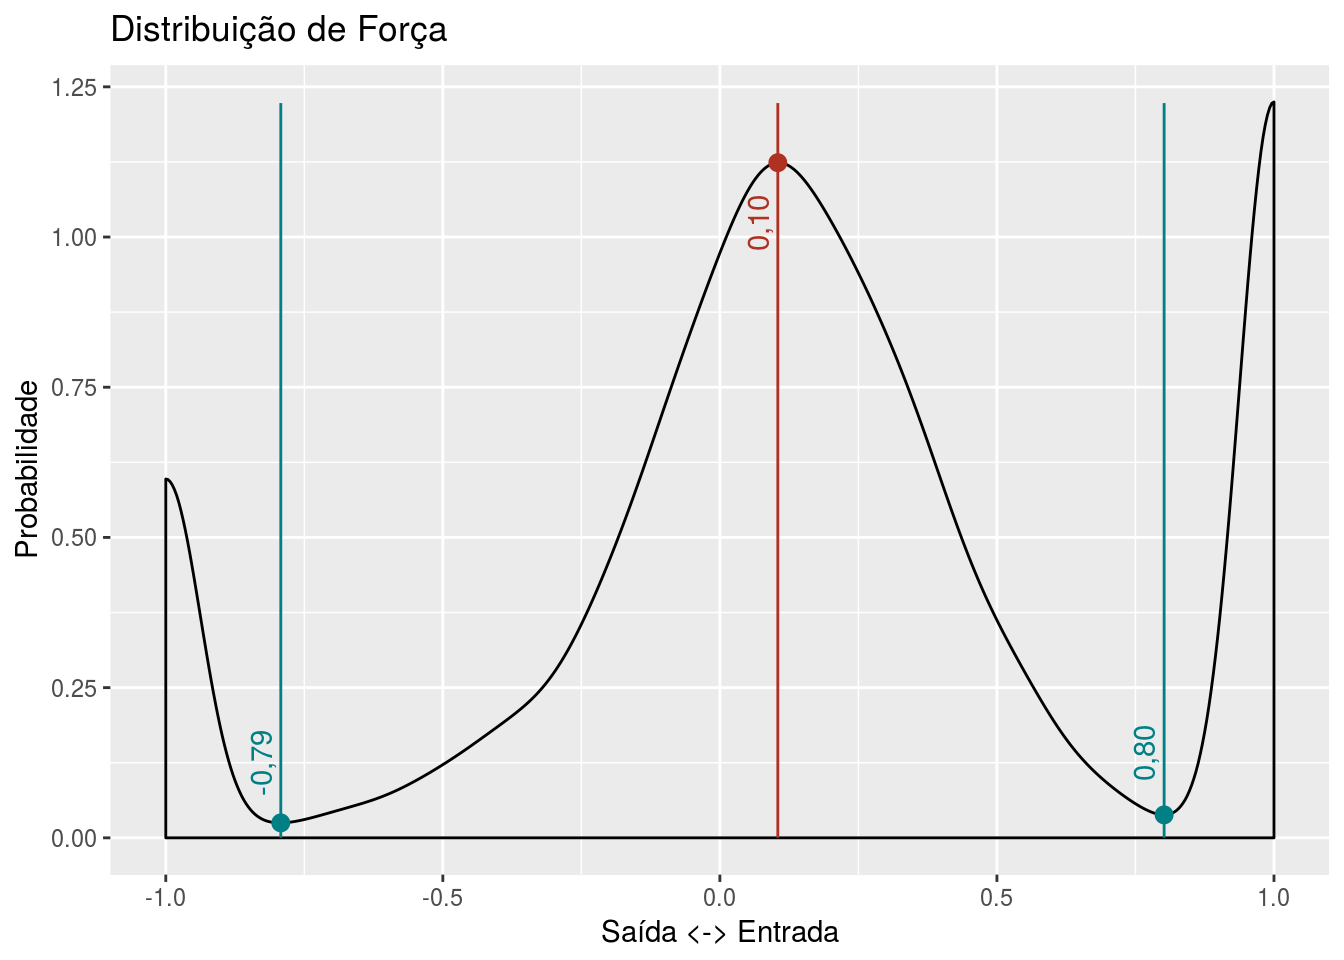
\includegraphics[scale=0.8]{distribuicao-de-forca.png}
    \caption{Distribuição de Força entre Ocupações}
    \label{fig:ditribuicao-de-forca}
\end{figure}

Na Figura~\ref{fig:ditribuicao-de-forca} é possível observar três picos (modas), dois deles nos extremos de antirreciprocidade e um próximo ao ponto mais recíproco. Os dois vales os separam claramente e podem ser usados como divisores, pois é onde a distribuição muda sua forma.

A porção mais negativa soma 712 nós e forma uma lista de ocupações mais comuns para ingressão no mercado de trabalho.

A porção mais positiva soma 1.437 nós e forma uma lista das ocupações mais comuns para evasão ou estagnação.

Analisando a lista de ocupações por amostragem, a explicação acima parece plausível. Por outro lado, as ocupações com pouca força de saída não parecem corresponder à hipótese.

A Tabela~\ref{tab:ocupacoes-de-ingresso} possui uma amostra de ocupações próximas ao ponto de separação entre pico de saída e o segundo pico.

\begin{table}[!h]
    \centering
    \begin{tabular}{l|r|r|r|r}
        \hline
        Ocupação & Força & Entrada & Saída & Fluxo\\
        \hline
        administrativo aprendiz jovem tecnico & 123 & 10 & 113 & -0.84\\
        \hline
        atendimento cliente profissional & 163 & 14 & 149 & -0.83\\
        \hline
        maquina moco & 138 & 12 & 126 & -0.83\\
        \hline
        embalador repositor & 143 & 13 & 130 & -0.82\\
        \hline
        equipe treinador & 185 & 17 & 168 & -0.82\\
        \hline
        aprendiz jovem mecanico & 135 & 13 & 122 & -0.81\\
        \hline
    \end{tabular}
    \caption{Ocupações de Ingresso}
    \label{tab:ocupacoes-de-ingresso}
\end{table}

Uma amostra de ocupações próximas ao ponto de separação entre o segundo pico e o pico de entrada é exibida na Tabela~\ref{tab:ocupacoes-de-evasao}.

\begin{table}[!h]
    \centering
    \begin{tabular}{l|r|r|r|r}
        \hline
        Ocupação & Força & Entrada & Saída & Fluxo\\
        \hline
        analista desenvolvimento pesquisa & 111 & 101 & 10 & 0.82\\
        \hline
        analista gestao & 113 & 103 & 10 & 0.82\\
        \hline
        analista commerce & 126 & 115 & 11 & 0.83\\
        \hline
        coordenador unidade & 121 & 111 & 10 & 0.83\\
        \hline
        consultor investimento & 152 & 142 & 10 & 0.87\\
        \hline
        fonoaudiologo & 181 & 170 & 11 & 0.88\\
        \hline
    \end{tabular}
    \caption{Ocupações de Evasão ou Estagnação}
    \label{tab:ocupacoes-de-evasao}
\end{table}

%% PARA CADA UMA DAS HIPÓTESES VOCÊ DEVE ILUSTRAR COM UMA FIGURA

\begin{hypothesis}[Trabalho de Passagem]
    Uma ocupação com alta centralidade de intermediação (Seção~\ref{sec:intermediacao}) significa um \enquote{trabalho de passagem}, em que um grande fluxo de profissionais passa por ela a caminho de outros trabalhos.
\end{hypothesis}

A Figura~\ref{fig:carreira-topografia} ilustra o conceito na carreira de topografia, onde o nó em destaque representa a ocupação com maior centralidade de intermediação. Essas ocupações merecem atenção especial no planejamento de carreira, pois são um ponto de convergência para ocupações que levam a ela e são pontos de difusão para as que partem dela.

\begin{figure}[ht]
  \centering
  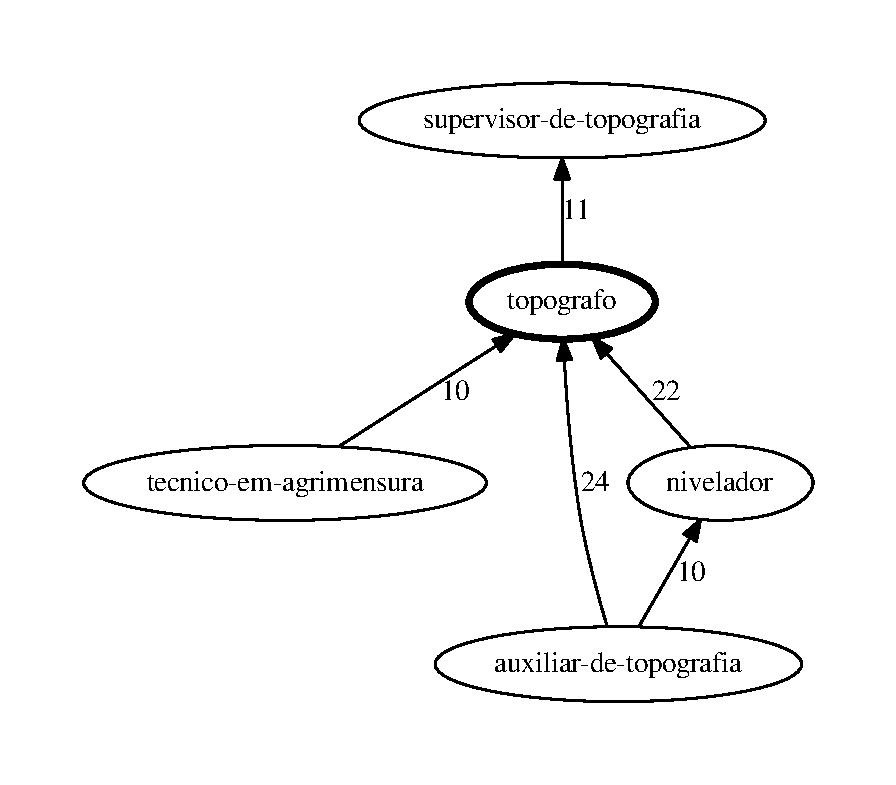
\includegraphics[scale=0.6]{cluster_25.pdf}
  \caption{Ilustração da centralidade de intermediação na carreira de topografia. O nó mais central é \enquote{topógrafo}.}
  \label{fig:carreira-topografia}
\end{figure}

NOTA: Aparentemente, essa hipótese não é válida para o grafo como um todo. Talvez para comunidades.

\begin{table}[!h]
    \centering
    \begin{tabular}{l|r|r}
        \hline
        & Intermediação & Normalizada\\
        \hline
        administrativo auxiliar & 9570434.6 & 0.2\\
        \hline
        vendedor & 3674933.3 & 0.1\\
        \hline
        administrativo assistente & 3541082.1 & 0.1\\
        \hline
        auxiliar producao & 2200145.0 & 0.0\\
        \hline
        recepcionista & 2158463.5 & 0.0\\
        \hline
        atendimento & 1628197.2 & 0.0\\
        \hline
        motorista & 1195781.9 & 0.0\\
        \hline
        analista suporte & 1095105.7 & 0.0\\
        \hline
        caixa operador & 1052277.6 & 0.0\\
        \hline
        analista sistema & 991204.4 & 0.0\\
        \hline
        maquina operador & 911173.1 & 0.0\\
        \hline
        professor & 901804.6 & 0.0\\
        \hline
        seguranca tecnico trabalho & 838408.0 & 0.0\\
        \hline
        analista humanos recursos & 799837.4 & 0.0\\
        \hline
        consultor venda & 780830.7 & 0.0\\
        \hline
    \end{tabular}
\end{table}


%% NESSA FIGURA VOCÊ PRECISA MOSTRAR O VALOR DA CENTRALIDADE DE INTERMEDIAÇÃO DE CADA NÓ, ASSIM VOCÊ MOSTRA QUANTITATIVAMENTE A DIFERENÇA.
\begin{hypothesis}[Equivalência Profissional] \label{hip:equivalencia}
    Em uma análise local, se $\recout{w}_{ij}$ é próximo de zero, ou se $\recout{w}_{ij} \ll \recboth{w}_{ij}$, então não há um sentido de \enquote{progressão} entre uma ocupação e outra, ou seja, profissionais vão e vêm entre elas sem uma preferência óbvia no fluxo, indicando que são equivalentes em termos profissionais.
\end{hypothesis}

A reciprocidade (Seção~\ref{sec:reciprocidade}) nessa pesquisa tem relação direta com o movimento entre ocupações. O peso recíproco $\recboth{w}_{ij}$ entre duas ocupações, em comparação com o peso não recíproco $\recout{w}_{ij}$, permite a compreensão do fluxo de pessoas pela rede. Derivando-se um grafo composto apenas por $\recout{w}_{ij}$ é possível observar a tendência de movimentação entre ocupações, ou seja, quais delas estão acumulando ou diminuindo o número de profissionais com o tempo.

Ao se analisar a reciprocidade global $\weighted{\rho}$ em componentes do MCar extraídos por agrupamento, é possível observar características de reciprocidade bastante distintas. Enquanto alguns componentes possuem alta reciprocidade, outros são claramente anti-recíprocos, sugerindo que há um caminho claro para os profissionais que se encontram naquele grupo.

\begin{hypothesis}[Detecção de Nomenclatura Equivalente]
    Se dois nós possuem similaridade máxima $\linkboth{S}(i,j) = 1$, ou seja, possuem exatamente os mesmos vizinhos, mas não há conexão entre eles, então esses nós são potencialmente nomenclaturas diferentes para a mesma ocupação.
\end{hypothesis}

Se duas ocupações possuem as mesmas entradas e saídas, mas não se conectam entre si, é um indício que elas na verdade são nomes diferentes para a mesma função. Entretanto, outros casos são possíveis, como ocupações que são paralelas em termos de progressão de carreira, mas não executam o mesmo trabalho. Por outro lado, se outros dados além da estrutura também forem similares, como a nuvem de palavras, essas ocupações são potencialmente nomenclaturas diferentes para a mesma função.
%% NESTE MOMENTO ME OCORRERAM DUAS POSSIBILIDADES DE APRESENTAÇÃO DESTE CAPÍTULO: 1) APRESENTAR INICIALMENTE PARTES DO MCar NAS QUAIS APARECEM OS CASOS DISCUTIDOS NAS HIPÓTESES; OU 2) APÓS CADA HIPÓTESE APRESENTAR EXEMPLOS NO MCar QUE ILUSTRAM (VALIDAM) AS HIPÓTESES.

\begin{hypothesis}[Capacitação Parcial] \label{hip:capacitacao-suficiente}
    O fluxo entre duas ocupações significa que parte das habilidades necessárias para se exercer a ocupação posterior está presente, ao menos em parte, nos profissionais da ocupação anterior.\todo{Existe o modelo CHA (Competência, Habilidade, Atitude) que talvez possa ser usado para expandir isso, se for conveniente.}
\end{hypothesis}

Se há uma movimentação entre profissionais de uma ocupação $a$ para uma ocupação $b$, significa que os profissionais de $a$ possuem capacitação, ao menos parcial, para exercer $b$. Esse conceito pode ser expresso mais precisamente considerando $\capac(x)$ como o conjunto de \textit{capacidades} para se exercer uma ocupação $x$, essa hipótese implica que $\capac(a) \cap \capac(b)  \ne \emptyset$ a menos que $\capac(b) = \emptyset$.

Usando a carreira de topógrafo da Figura~\ref{fig:carreira-topografia} como exemplo, o \textit{Nivelador} possui um subconjunto das capacidades para exercer a função de \textit{Topógrafo}, esse subconjunto não deve ser vazio a menos que a ocupação de \textit{Topógrafo} não exija nenhuma capacitação.

\begin{hypothesis}[Identificação de Carreiras]
    Uma comunidade dentro do MCar significa que o fluxo de profissionais dentro desse grupo é maior do que com outros nós, indicando que é um conjunto de ocupações que pode ser exercido por profissionais com capacitações em comum (Hipótese~\ref{hip:capacitacao-suficiente}). Se a comunidade possui uma direção de fluxo óbvio entre as ocupações, isso indica progressão (Hipótese~\ref{hip:equivalencia}). Ambas as propriedades presentes caracterizam uma carreira.
\end{hypothesis}


\section{CRONOGRAMA}

Aqui apresentamos um panorama resumido de como o trabalho evoluiu até o momento e como é esperado seu desenvolvimento até sua entrega.

Os dados que são fonte para a pesquisa estão prontos e no formato adequado, nenhum processamento extra é necessário nesse ponto. A descrição de como ele é obtido está concluída, sendo necessário apenas ajustes para uma melhor compreensão do texto e detalhes menores na descrição da estrutura dos dados. Grande parte dos meses de Fevereiro e Março foram usados na elaboração do texto e aparecem no cronograma da Figura~\ref{fig:cronograma} descritos como \textit{Descrição da Fonte de Dados}.

Os conceitos de Ciência de Redes suficientes para esse trabalho já estão absorvidos e o referencial teórico está quase completamente escrito. Ainda falta uma elaboração melhor do texto para facilitar a compreensão dos algoritmos dos modelos nulos, mas é previsto que até o final de Junho esses ajustes estejam concluídos.

A metodologia da pesquisa também está definida e descrita no trabalho. Por outro lado, é provável que durante o início dos experimentos, mais material precise ser estudado e adicionado a ele, bem como ajustes na metodologia, mas espera-se que ao final de Agosto a pesquisa esteja consolidada o suficiente para que nenhuma nova adição seja necessária. São esperadas apenas alterações esporádicas no texto para refletir essa consolidação. No cronograma da Figura~\ref{fig:cronograma}, essas etapas estão descritas como \textit{Referencial Teórico} e \textit{Metodologia}.

A partir do final de Junho iniciam os experimentos. A maior parte dos modelos nulos e medições necessárias já existem em bibliotecas nas linguagens R e Python, o que acelera a experimentação. Entretanto, há trabalho de codificação de algoritmos a ser feito, pois nem todos os modelos estão disponíveis em bibliotecas. Como a fonte de dados do trabalho é um grafo direcionado e ponderado e a literatura é escassa para esse tipo de rede, alguns modelos e medições adaptadas foram propostas, o que significa que seus algoritmos precisam ser implementados computacionalmente. Dada a experiência do pesquisador com desenvolvimento de software, espera-se que essas implementações junto com a própria experimentação não ultrapasse Setembro. No cronograma da Figura~\ref{fig:cronograma} essa etapa é descrita como \textit{Experimentação}. A implementação dos algoritmos e a experimentação não são separadas no cronograma pois espera-se que ocorram concomitantemente.

Uma vez que os primeiros resultados forem obtidos, espera-se começar sua consolidação e transferência para o trabalho escrito. Essa etapa deve acontecer esporadicamente enquanto a atividade principal da experimentação ocorre. É esperado que os experimentos já estejam concluídos até Outubro e que esse mês seja quase totalmente reservado na descrição dos resultados. No cronograma da Figura~\ref{fig:cronograma} a etapa como um todo recebe o nome de \textit{Descrição dos Resultados}.

Finalmente, as revisões finais do trabalho devem começar timidamente em Outubro, quando os resultados forem confrontados com o que foi descrito até o momento. Novembro é reservado para ajustes de texto causados pelo resultado dos experimentos e melhorias na redação. No cronograma da Figura~\ref{fig:cronograma} essa etapa final é chamada \textit{Consolidação do Trabalho}.

\begin{figure*}[htb]
    \centering
    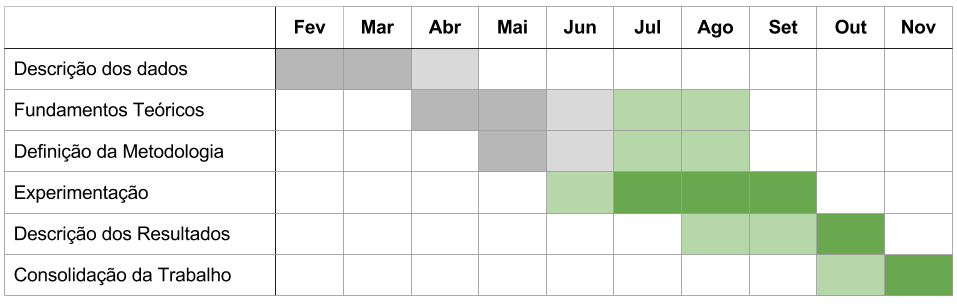
\includegraphics[scale=0.4]{dissertacao-cronograma.png}
    \caption{Cronograma}
    \label{fig:cronograma}
\end{figure*}

\begin{comment}
\section{Geladeira}

Aqui fica o texto escrito e que pode ser reaproveitado em outras partes do trabalho, mas que parece que não encaixa de onde foram tirados.


\subsection{Análise de classe de ocupações}

Uma coisa que reparei enquanto montava o MCar (olhei para aqueles dados por bastante tempo) é que temos 4 tipos de trabalho que não se misturam muito. Abaixo uma descrição \enquote{no cheiro} do que observei, mas precisa de algo melhor para realmente embasar as observações abaixo.


\begin{description}
\item [Operacional] Escolaridade no 3º grau incompleto (ou menor, 2º grau é o mais comum. Contém \enquote{graduações saturadas} como Direito e Administração de Empresas. Salário é mais baixo. Grande migração entre outros cargos operacionais sem muita correlação (garçom → mascote esportivo → pedreiro → lavador de carro → manobrista → recepcionista). Parece haver uma subdivisão aqui entre operacional de escritório (recepcionista, auxiliar administrativo, \ldots) e operacional \textit{braçal} (manobrista, lavador, garçom, \ldots) Os operacionais de escritório parecem ter níveis de experiência divididos entre \enquote{Assistentes} e \enquote{Auxiliares}.
\item [Técnico] Com algumas migrações vindas do operacional. Possui 3º grau incompleto ou menor. È bastante similar ao Operacional, mas os salários são um pouco maiores e a movimentação entre cargos não correlacionados diminui. Possui níveis de experiência: \enquote{Meio Oficial} e \enquote{Oficial}. Exemplos: Soldador, Enfermeiro, Mecânico, Cozinheiro, \ldots
\item [Especialista] Com 3º completo e acima (mestrado e doutorado são mais comuns). Possui pouquíssima movimentação para ocupações não correlacionadas, exceto para área de gestão. Possui níveis de experiência \enquote{Júnior}, \enquote{Pleno} e \enquote{Sênior}. Salários são maiores. Descrição nos currículos normalmente possui habilidades e ferramentas. Exemplos: Desenvolvedores de Software, Médicos, Arquitetos, Engenheiros (todos), \ldots
\item [Gestores] Com variados graus de formação, mas os de maior salário (ou empresas maiores) possuem formação superior ou acima (especializações e MBA são mais comuns). Pouca movimentação entre cargos não correlacionados. Salários são maiores. Classificação de experiência parece ser \enquote{Supervisor}, \enquote{Coordenador}, \enquote{Gerente}, \enquote{Diretor}. Recentemente aparecem \enquote{CEO}, \enquote{CFO}, entre outros \enquote{C's}.
\end{description}

Na minha humilde opinião, esse á um trabalho que seria uma contribuição interessante para a área de RH, pois o que descrevo aí embaixo parece ser algo formalizado pela área (provavelmente), mas que poderia ganhar bases sólidas com uma análise com esse volume de dados. Um ponto particularmente interessante é que não existe uma migração muito forte de uma para o outro, ao contrário do que já vi descrito por aí: operacional → técnico → especialista → gestão. O que parece existir é uma migração muito grande dentro de cada grupo. O operacional é mais \enquote{bagunçado}, não existe um ordem, enquanto existe uma clara progressão nos outros. Também existe uma migração de Operacional para Técnico, mas quase zero de Técnico para Especialista.

\subsection{Identificação de \textit{Carreiras}}

Basicamente a clusterização já feita para separar o subgrafo da área de TI.

Existe um desafio ali que são as ocupações \enquote{hubs} que conectam tudo (vendedor, recepcionista, auxiliar administrativo).

O grupo dos cargos operacionais é muito grande e pode ser dividido.

A técnica que usei foi simples. Separar os clusters e passar novamente o algoritmo nos maiores com parametrização mais rígida (dá para automatizar esse processo). Porém sobrou o problema dos \enquote{miniclusters} com duas ou três ocupações que poderiam se juntar à outras.

Seria possível aplicar outras técnicas de agrupamento.
\end{comment}

\def\refname{REFERÊNCIAS BIBLIOGRÁFICAS}
\bibliography{main}
\addcontentsline{toc}{section}{REFERÊNCIAS BIBLIOGRÁFICAS}
\bibliographystyle{abnt-alf}

\end{document}
